%-------------
%-------------
% \documentclass[prl,amsfonts,showpacs]{revtex4}
%
%\documentclass[aps,amsfonts,prl,twocolumn,showpacs]{revtex4}
%
%\documentclass[preprint,amsfonts,showpacs]{revtex4}
%\documentclass[aps,amsfonts,pra,twocolumn,showpacs,eqsecnum]{revtex4}
%\usepackage{amsmath,amssymb,bm,epsfig,epsf,graphics,verbatim}
\documentclass[nottitlepage]{article}
\usepackage{amsmath,amssymb,bm,epsfig,graphics,verbatim}
\usepackage{breqn}
\usepackage{geometry}
\geometry
{
letterpaper,
top=1in,
bottom=1in,
left=1in,
right=1in,
}
\usepackage[usenames,dvipsnames]{color}
\usepackage{amsfonts}
\usepackage{mathrsfs}
\usepackage{graphicx}
%\usepackage[margin=10pt,font=small,labelfont=bf,justification=centering]{caption}
%\usepackage{lipsum}
\usepackage{caption}
\usepackage{subcaption}
\usepackage{tikz}
\usepackage{pgfplots}
%\documentclass{report}
\setcounter{secnumdepth}{3}
\graphicspath{{./Pictures/}}

%\usepackage{hyperref}
\usepackage{cleveref}
\crefname{section}{Sec.}{Secs.}

\providecommand\hyperref[2][]{#2}

\makeatletter
\newcommand{\mt@ref}[1]{%
\cref@gettype{#1}{\@temptype}%
\cref@getcounter{#1}{\@tempctr}%
\def\mtt{\the\csname c@\@temptype\endcsname}%
\ifnum\mtt=\numexpr\@tempctr-1\relax \mtcase the next \hyperref[#1]{\@temptype}\else%
\ifnum\mtt=\numexpr\@tempctr+1\relax \mtcase the previous \hyperref[#1]{\@temptype}\else%
\cref{#1}\fi\fi}

\newcommand{\mtref}{\let\mtcase\relax\mt@ref}
\newcommand{\Mtref}{\let\mtcase\MakeUppercase\mt@ref}
\makeatother


\begin{document}
%-------------
%-------------

\title{Topological Defects in Liquid Crystals
\\and Transitions Between Them}

\author{Shengnan Huang\\
\\
\multicolumn{1}{p{.8\textwidth}}{\centering\emph{School of Physics, Georgia Institute of Technology,
\\837~State Street, Atlanta, GA~30332}}}

%-------------
\date{\today}
%\date{** April 23, 2013}
%\pacs{**}
%{**}
\maketitle

\begin{abstract}
In this paper, basic theories of liquid crystals and defects are reviewed. Difficulties regarding a quantitative study of the defects in a closed cylinder and a nematic bridge are discussed. The current research is reviewed, and our future work is proposed.
\end{abstract}






\section {Introduction: Liquid crystals}

Liquid crystals, whose basic microscopic components are rod-like or disc-like molecules, exhibit unusual emergent phenomena in which spatial and orientational correlations present over short distances may or may not fade away at large distances. In this sense, they are partially reminiscent of liquids and solids. Distinct phases of liquid crystals include isotropic, nematic, cholesteric, smectic and columnar. As a result of their different order, they have distinct elastic, electric and optical properties; see Refs.~\cite{Mottram, de gennes}. %Successful theories are the Onsager model (for lyotropic liquid crystals), the Maier-Saupe theory (for thermotropic liquid crystals), and the Landau-de Gennes' phenomenological theory \cite{de gennes}. The last one is most widely used for its simplicity and effectiveness in dealing with different types of phase transitions.

%The phases are characterized by the molecular ordering. Given a local region, if on average, the rod-loke molecules are aligned along one axis or the disc-like molecules are perpendicular to that axis, then the order can be described by a unit vector indicating the orientation of the axis i.e., $\mathbf{n}$ ($|\mathbf{n}|=1$) with head-tail symmetry (i.e., $\mathbf{n}=-\mathbf{n}$), and the system is in the uniaxial phase. $\mathbf{n}$ is called the director, a local average of the orientations of molecules (not the molecule itself). If the arrangement of the molecules is biaxial, then two unit vectors $\mathbf{n}$ and $\mathbf{m}$ are needed, with the symmetry $\mathbf{n}=-\mathbf{n}$, $\mathbf{m}=-\mathbf{m}$. Uniaxial and biaxial arrangements can both be described by a tensor order parameter \cite{Mottram}:

%\begin{equation} \label{eq:Q}
%\mathbf{Q}=S_1\mathbf{n}\otimes \mathbf{n}+S_2\mathbf{m}\otimes \mathbf{m}-\frac{1}{3}(S_1+S_2)\mathbf{I}
 %\end{equation}
%where $\mathrm{Tr}(\mathbf{Q})=0$, and $S_1$, $S_2$ are eigenvalues. %Compared with the complex order parameter of the superconductor, $S_1$, $S_2$ can be regarded as the ``amplitudes", and $\mathbf{n}\otimes \mathbf{n}$, $\mathbf{m}\otimes \mathbf{m}$ are the ``phase angles".
%Even though $\mathbf{Q}$ is the correct parameter to study the phase transitions or the coexistence of multiple phases in liquid crystals, the director field $\mathbf{n}$ is more conveniently used if the system is solely in the uniaxial (nematic) phase as well as the director field is orientable.

% %Isotropic and nematic
Phases, such as isotropic and nematic, whose translational symmetry is maintained while the rotational symmetry may or may not be broken, can be characterized by the order parameter $\mathbf{Q}$, which is a symmetric traceless tensor field and can be represented by a $3\times 3$ matrix, which can be diagonalized as 

\begin{equation}\label{eq:Q111}
\mathbf{Q}=\frac{1}{3}
  \begin{bmatrix}
    2S_1-S_2 & 0 & 0  \\
    0 & -S_1-S_2 & 0 \\
    0 & 0 & -S_1+2S_2
  \end{bmatrix},
\end{equation}
where $S_1$ and $S_2$ are scalar fields; see Refs.~\cite{Mottram, de gennes, lubensky}. If the system is in the isotropic phase then $\mathbf{Q}=0$, i.e., $S_1=S_2=0$. If it is in the uniaxial nematic phase then $S_1\neq 0$, $S_2=0$,  and $\mathbf{Q}$ simplifies to
\begin{equation} \label{eq:Q22}
\mathbf{Q}=S\,(\mathbf{n}\otimes \mathbf{n}-\frac{1}{3}\mathbf{I}),
 \end{equation}
 and in terms of Cartesian coordinates, it becomes
\begin{equation}\label{eq:Q}
Q_{ij}=S \,(n_i\,n_j-\frac{1}{3}\delta_{ij}),
\end{equation}
where $i$, $j$ are Cartesian indices, $\delta_{ij}$ is the Kronecker delta, $S$ is a scalar field, and $\mathbf{n}$ is a unit vector field, also known as the director field \cite{de gennes}. The scalar field $S$ is a second moment average of the distribution of the orientations of the molecules near some particular spatial point $\mathbf{r}$ and it is defined as
\begin{equation}\label{eq:Q2}
S(\mathbf{r})=\frac{1}{2}\langle 3\cos^{2}\theta-1\rangle=\frac{1}{2}\int (3\cos^{2}\theta-1)f(\theta,\mathbf{r})\mathrm{d}\theta,
 \end{equation}
where $\langle\cdots\rangle$ is a statistical-mechanical average, $\theta$ is the angle between $\mathbf{n}$ and the orientation of each molecule, and $f(\theta,\mathbf{r})$ is the distribution of the $\theta$ near the point $\mathbf{r}$, which satisfies $f(\theta,\mathbf{r})=f(\pi-\theta,\mathbf{r})$ because $\mathbf{n}$ and $-\mathbf{n}$ represent the same local direction of molecular alignment (i.e., head-tail symmetry). %implying the head-tail symmetry of $\mathbf{n}$.
If the molecules are fully oriented in some particular direction then $S=1$;   if the molecules are fully randomly oriented in $3$-dimensional space (so that the system is in an isotropic phase) then $S=0$; and if the molecules are fully randomly oriented in an $2$-dimensional plane perpendicular to some axis then $S=-1/2$; see Refs.~\cite{Mottram, de gennes}. %This information is particularly useful for picturing the core structures of the defects in liquid crystals.


If the system is, however, in the {\it biaxial} nematic phase then $S_1\neq 0$ and $S_2\neq 0$. Equation (\ref{eq:Q111}) can be written compactly as

\begin{equation} \label{eq:Q11}
\mathbf{Q}=S_1\,\mathbf{n}\otimes \mathbf{n}+S_2\,\mathbf{m}\otimes \mathbf{m}-\frac{1}{3}(S_1+S_2)\,\mathbf{I},
 \end{equation}
 or equivalently,
\begin{equation}\label{eq:Q2}
Q_{ij}=S_1\,n_i\,n_j+S_2\,m_i\,m_j-\frac{1}{3}(S_1+S_2)\,\delta_{ij},
\end{equation}
where $\mathbf{m}$ is a unit vector field perpendicular to $\mathbf{n}$ \cite{Mottram}.


\subsection { %The Scalar Field $S$ in Characterizing the Isotropic Phase and the Uniaxial Nematic Phase %
Isotropic-Nematic Phase Transition}
%Given a system that can be in either the isotropic phase or the nematic phase, the amplitude of the thermally averaged order parameter is \cite{Mottram}\cite{de gennes}:

When the temperature of the system is close to the isotropic-nematic transition temperature, the bulk free energy density $\mathcal{F}_b$ can be expanded in: ($a$) powers of $\mathbf{Q}$, and ($b$) gradients of $\mathbf{Q}$. The reason of ($a$) is that the order parameter $\mathbf{Q}$ is typically rather small despite the discontinuous character of the transition, while ($b$) represents the energy cost due to the long-wavelength spatial distortion of the equilibrium states which are assumed to be spatially uniform \cite{de gennes}.

Therefore, to determine the equilibrium states below and above the transition point, we can ignore ($b$) and express $\mathcal{F}_b$  as

\begin{equation}\label{eq:F3}
\mathcal{F}_{b}=\frac{3}{2}a(T-T^{*})\, \mathrm{Tr}(\mathbf{Q}^2)-\frac{9}{2}b\mathrm{Tr}(\mathbf{Q}^3)+\frac{9}{4}c\mathrm{Tr}(\mathbf{Q}^4),
\end{equation}
where $a$, $b$, $c$ and $T^{*}$ are approximately independent of temperature and pressure. $\mathcal{F}_{b}$ is known as the Landau-de Gennes free energy density; see Refs.~\cite{Mottram, and}.

Assuming that the nematic phase is uniaxial, Equation~(\ref{eq:F3}) becomes (by using Eq.~(\ref{eq:Q22}))

\begin{equation}\label{eq:F333}
\mathcal{F}_{b}=a(T-T^{*}) S^2-bS^3+cS^4.
\end{equation}
At the transition temperature $T_p=T^{*}+b^2/ac$, the scalar field has the value for $S_p=b/2c$. For the common nematic material 5CB, one has $a\approx 5.2\times 10^{4}{\rm J\/}{\rm m\/}^{-3}{\rm K}^{-1}$, $b\approx 5.3\times 10^5{\rm J\/}{\rm m\/}^{-3}$, $c\approx 9.7\times 10^{5}{\rm J\/}{\rm m\/}^{-3}$, $T^*\approx 307.55{\rm K}$, and $T_p\approx 308.94{\rm K}$, $S_c\approx 0.27$ \cite{nita}.




%This example is simple because this tensor $\mathbf{Q}$ is  unable to describe the biaxial phase. It is not too simple in that we cannot use the director $\mathbf{n}$ instead of $\mathbf{Q}$. $\mathbf{n}$ is not naturally equipped with the head-tail symmetry, therefore works awkwardly in confined geometry where the director field may be non-orientable.
\subsection {Order Parameter of the Uniaxial Nematic Phase in the Low-Temperature Regime}\label{sssec:uniaxial}
The uniaxial nematic phase is the simplest example of a liquid crystal phase having nontrivial (i.e., nonzero) order parameter. In the low-temperature regime (in which the temperature is much lower than the nematic-isotropic transition temperature), fluctuations of $S$ are weak, therefore the part of the free energy density contributed by $S$ is approximately a constant, while the part that contributed by the gradients of $\mathbf{Q}$ or $\mathbf{n}$, i.e., the (long-wavelength) distortion free energy density, is dominated by the lowest gradients allowed by symmetry. With few parameters, this argument simplifies the description of the low-temperature phase.

Let me digress to make a point that is sometimes overlooked. Unlike $\mathbf{Q}$, the director field $\mathbf{n}$ is not an order parameter. Rather, $\mathbf{n}$ and $-\mathbf{n}$ equivalently characterize the local direction of molecular alignment. Taken alone, $\mathbf{n}$ or $-\mathbf{n}$ hide the head-tail symmetry. In some cases, $\mathbf{n}$ cannot replace $\mathbf{Q}$ without flipping through $\pi$ rad on some lines or planes.
%However, compared with $\mathbf{Q}$, $\mathbf{n}$ is devoid of the head-tail symmetry, i.e., $\mathbf{n}=-\mathbf{n}$, therefore it is not a proper order parameter if it has to flip $180^{\circ}$ at some points.
%There is a fact that the tensor field $\mathbf{Q}$ cannot always be replaced by a director field $\mathbf{n}$ without creating such discontinuities \cite{ball}.
To illustrate this situation, we use ``arrows" and ``sticks" to represent $\mathbf{n}$ and $\mathbf{Q}$, respectively, in schematic diagrams. 
%The above director field $\mathbf{n}$ and tensor field $\mathbf{Q}$ have the same local property, i.e., changes of the orientation in the nearby regions are the same for both of them%, which implies that free energy densities in terms of $\mathbf{n}$ or $\mathbf{Q}$ are equivalent for the low temperature uniaxial nematic phase
%. However, they are globally different and not all tensor fields can be replaced by director fields without creating discontinuities \cite{ball}.
%Once we know the director field, to further investigate the orientation change in the nearby local region, it is convenient to replace the director field (with head-tail symmetry) by a vector field (with no head-tail symmetry).
Figures~\ref{fig:tensordirector1} and \ref{fig:tensordirector2} illustrate the tensor fields and their corresponding director fields assuming homeotropic boundary conditions (i.e., $\mathbf{n}$ is perpendicular to the boundary). The former represents a state where both $\mathbf{n}$ and $\mathbf{Q}$ are continuous, while the latter is a state where $\mathbf{n}$ inevitably flips through $\pi$ rad on a line %while vectors rotate at most $90^{\circ}$ at some points in Fig. \ref{fig:orientable}
while the corresponding $\mathbf{Q}$ is continuous. %In contrast, no such discontinuities are created in Fig.~\ref{fig:orientable}. %A rigorous mathematical analysis is elaborated in \cite{ball}.
%The director fields corresponding to Figs.~\ref{fig:orientable} and ~\ref{fig:nonorientable} are examples of orientable and non-orientable director fields respectively \cite{ball}. Therefore, for the uniaxial nematic phase with an orientable director field, it is convenient to use the vector field representation in the calculations.
%If we use the free energy in terms of $\mathbf{n}$, these discontinuities can cost unphysical free energy.


% $\mathbf{n}$ and $\mathbf{m}$ represent the local averages of the molecular ordering. Take the uniaxial nematics for example, given a local region, on average, the rod-loke molecules are aligned along one axis or the disc-like molecules are perpendicular to that axis, $\mathbf{n}$ is the orientation of the axis

%The director field $\mathbf{n}$ is more conveniently used if the system is  in the uniaxial nematic phase as well as the director field is orientable.
%\begin{figure}
%\centering
%\begin{subfigure}{.4\textwidth}
 %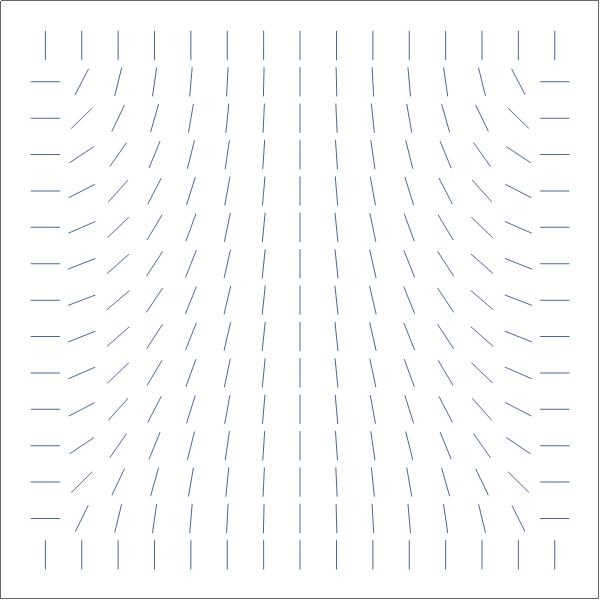
\includegraphics[scale=0.3]{orientabletensor.jpg}
 %  \caption{Uniaxial tensor field  \#1}
 % \label{fig:orientabletensor}
%\end{subfigure} %
%\hfill
%\begin{subfigure}{.4\textwidth}
 %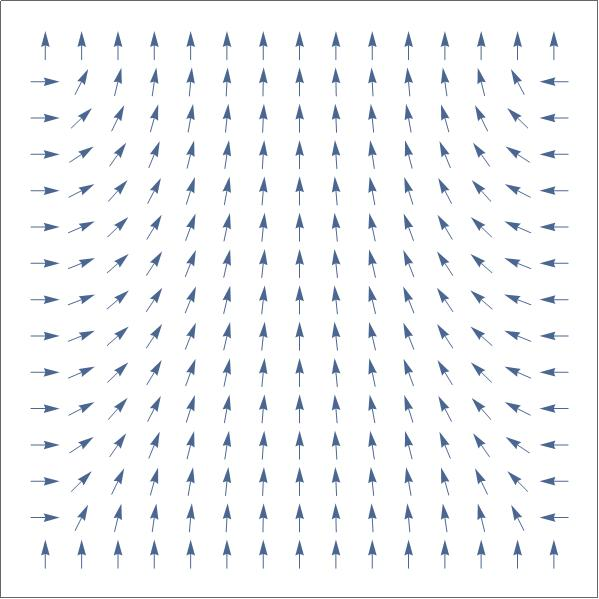
\includegraphics[scale=0.3]{orientable2.jpg}
 %\caption{Director field \#1 (no vector flips $\pi$ rad)}
%  \label{fig:orientable}
%\end{subfigure}
%\caption{Uniaxial tensor field \#1 (left) and its corresponding director field \#1 (right), for the case in which there are no topological defects.}
%\label{fig:tensordirector1}
%\end{figure}


%\begin{figure}
%\centering
%\begin{subfigure}{.4\textwidth}
 %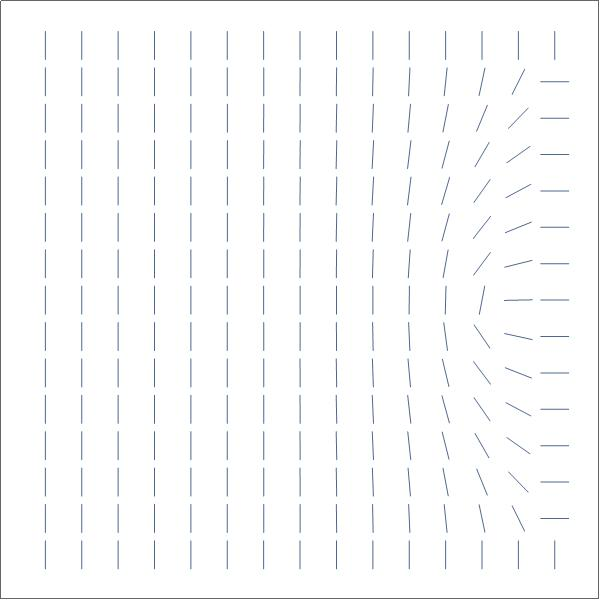
\includegraphics[scale=0.3]{nonorientabletensor.jpg}
 %  \caption{Uniaxial tensor field \#2}
  %\label{fig:nonorientabletensor}
%\end{subfigure} %
%\hfill
%\begin{subfigure}{.4\textwidth}
 %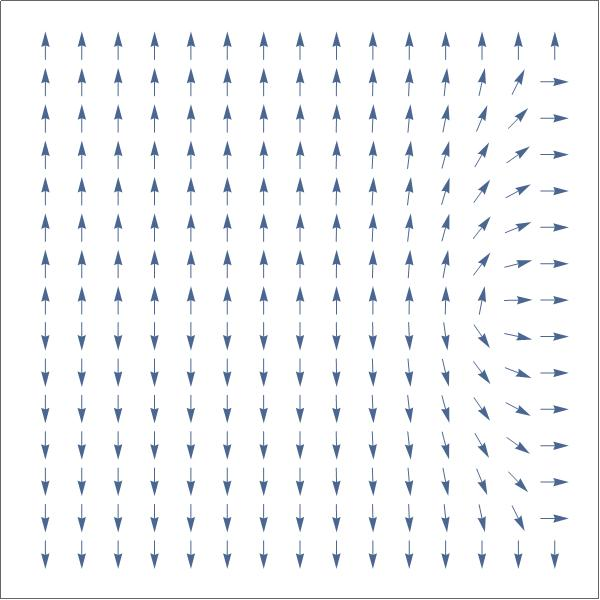
\includegraphics[scale=0.3]{nonorientable2.jpg}
% \caption{Director field \#2 (some vectors flip $\pi$ rad)}
  %\label{fig:nonorientable}
%\end{subfigure}
%\caption{Uniaxial tensor field \#2 (left) and its corresponding director field \#2 (right), for the case in which there is a topological defect.}
%\label{fig:tensordirector2}
%\end{figure}


%Whether the director field is orientable or non-orientable depends on the





%\section {Uniaxial Nematic Phase in the Low-Temperature Regime}

%Near the isotropic-uniaxial nematic phase transition, the amplitude of the order parameter $\mathbf{Q}$ is small, the free-energy density $\mathcal{F}_b$ can be expanded in powers of $\mathbf{Q}$ and its gradients. In the low-temperature regime (in which the temperature is much lower than the nematic-isotropic transition temperature), fluctuations of $S$ are small, and therefore $S$ is approximately independent of the spatial position, and $\mathbf{Q}$ has the same number of degrees of freedom as $\mathbf{n}$. Therefore, the amplitude part is always a constant and can be ignored, while the gradient part is contributed mainly by the lowest order terms, i.e., Goldstone fluctuations. With few parameters, this argument simplifies the description of the low temperature phase.

\subsection {Elasticity of the Uniaxial Nematic Phase in the Low-Temperature Regime}

%The Landau-de Gennes free energy $F$ can be separated into the bulk free energy $F_b$ and the distortion free energy $F_d$:

%\begin{equation}\label{eq:F}
%F=\int \mathcal{F}_1\mathrm{d}V+\int \mathcal{F}_2\mathrm{d}S
%\end{equation}
%\begin{equation}\label{eq:F}
%F=F_b+F_d
%\end{equation}
%where
%\begin{equation}\label{eq:F111}
%F_b=\int\mathcal{F}_b\mathrm{d}V
%\end{equation}
%\begin{equation}\label{eq:F112}
%F_d=\int\mathcal{F}_d\mathrm{d}V
%\end{equation}

The distortion free energy density $\mathcal{F}_b$ consists of the lowest gradients of $\mathbf{Q}$ that are symmetry-invariant. In general, for the uniaxial or biaxial nematic phase in the low-temperature regime, $\mathcal{F}_b$ can be expressed as
\begin{equation}\label{eq:F4}
\mathcal{F}_{d}=\frac{L_1}{2}(\frac{\partial Q_{ij}}{\partial x_{k}})^2+\frac{L_2}{2}\frac{\partial Q_{ij}}{\partial x_{j}}\frac{\partial Q_{ik}}{\partial x_{k}}+\frac{L_3}{2}\frac{\partial Q_{ik}}{\partial x_{j}}\frac{\partial Q_{ij}}{\partial x_{k}}+
%\frac{L_4}{2}\epsilon_{lik}Q_{lj}\frac{\partial Q_{ij}}{\partial x_{k}}+
\frac{L_6}{2}Q_{lk}\frac{\partial Q_{ij}}{\partial x_{l}}\frac{\partial Q_{ij}}{\partial x_{k}},
\end{equation}
where $L_1$, $L_2$, $L_3$ and $L_6$ are constants.
%For the nematic phase in the low temperature regime (either uniaxial or biaxial), $S$, $S_1$, $S_2$ are approximately constants. As a result, at a specific temperature $T$, $\mathcal{F}_{b}$ is a constant, and $\mathcal{F}_{d}$ alone can be used to study the distorted nematic phase.
For the uniaxial nematic phase in the low temperature regime, $\mathcal{F}_{d}$ can be expressed in terms of $\mathbf{n}$ (provided that $\mathbf{n}$ is ``as smooth as" $\mathbf{Q}$):


\begin{dmath}\label{eq:F5}
\mathcal{F}_{d}=\frac{K_{11}}{2}(\nabla \cdot \mathbf{n} )^2+\frac{K_{22}}{2}(\mathbf{n}\cdot(\nabla\times\mathbf{n}) )^2+ \frac{K_{33}}{2}(\mathbf{n}\times(\nabla\times\mathbf{n}) )^2-K_{24}\nabla\cdot[(\mathbf{n}\times(\nabla\times\mathbf{n})+\mathbf{n}(\nabla \cdot \mathbf{n}))], %+K_{13}\nabla\cdot[(\mathbf{n}(\nabla \cdot \mathbf{n}))]
%\\-\frac{K_{24}}{2}(\mathbf{n}\times\nabla\times\mathbf{n}+\mathbf{n}\nabla \cdot \mathbf{n})\cdot\mathbf{v}\delta(\mathbf{r}-\mathbf{R})+K_{13}(\mathbf{n}\nabla \cdot \mathbf{n})\cdot\mathbf{v}\delta(\mathbf{r}-\mathbf{R})
\end{dmath}
%The free energy density $\mathcal{F}_2$ is written as \cite{zumer}\cite{per}:
%\begin{equation}\label{eq:F6}
%\mathcal{F}_2=-K_{24}[(\mathbf{n}\times(\nabla\times\mathbf{n})+\mathbf{n}(\nabla \cdot \mathbf{n}))]\cdot \nu+K_{13}[(\mathbf{n}(\nabla \cdot \mathbf{n}))]\cdot\nu
%\end{equation}
%where $\nu$ is the normal vector of the boundary.
%Eqs.~(\ref{eq:F5}) is called Frank free energy density \cite{oseen}\cite{frank}.
where the four terms represent respectively, the contributions of the splay, twist, bend and saddle-splay; see Refs.~\cite{Mottram, zar, berreman, mori2, zumer}. A term corresponding to the contribution of splay-bend, i.e.,

\begin{equation}\label{eq:splay}
K_{13}\nabla\cdot[\mathbf{n}(\nabla \cdot \mathbf{n})],
\end{equation}
is beyond the scope of this article. %with the last two being surface free energies.
%Since there are confusions about the splay-bend, we will focus on the other four terms. %Note that the vectorial representation only works for uniaxial phase, therefore has more limited use than the tensorial one.
%It is easy to show that these five terms are enough describe the distortion whether the deformation is large or small. In addition,
%It has been proved that, in describing the uniaxial nematic phase, both Eq.~\ref{eq:F4} and Eq.~\ref{eq:F5} exhaust all the possible terms \cite{berreman}\cite{trebin}.

The saddle-splay term can be written, using the divergence theorem, as a surface integral

\begin{equation}\label{eq:splay2}
-\int K_{24}[\mathbf{n}\times(\nabla\times\mathbf{n})+\mathbf{n}(\nabla \cdot \mathbf{n})]\cdot\mathbf{v}\mathrm{d}S,
\end{equation}
where $\mathbf{v}$ is the vector normal to the boundary. This term does not contain any derivatives of $\mathbf{n}$ in the normal direction of the boundary; see Refs.~\cite{per, fati}. Therefore, it is a constant when the boundary conditions are given and Eq.~(\ref{eq:F5}) simplifies to
\begin{equation}\label{eq:F555}
\mathcal{F}_{d}=\frac{K_{11}}{2}(\nabla \cdot \mathbf{n} )^2+\frac{K_{22}}{2}(\mathbf{n}\cdot(\nabla\times\mathbf{n}) )^2+ \frac{K_{33}}{2}\left|\mathbf{n}\times(\nabla\times\mathbf{n}) \right|^2.
\end{equation}

\section {Equilibrium States of Topological Defects in Nematics}
\label{sssecc:topo}
The director field $\mathbf{n}$ captures the long-wavelength physics of nematics. In this description, the topological defects can be characterized by $\mathbf{n}$ changing discontinuously, and their defect cores lie in the singular regions with internal structures being ignored. In contrast, the defect core is difficult to  be determined in the tensor-field description, since $\mathbf{Q}$ is always continuous throughout the whole region. Based on the dimensionality of the cores, there are point and line  defects (note that the closed line is called a ring). The latter includes two simple types: wedge and twist disclination. For the point or ring defects, there are radial and hyperbolic types: the former is characterized by $\mathbf{n}$ pointing mainly in the radial direction from the core, and the latter can be obtained by inverting one component of $\mathbf{n}$ in the radial type; see Refs.~\cite{de gennes, zar, luca, paul2}.


To determine the equilibrium state of defects (i.e., the spatial configuration of $\mathbf{Q}$ or $\mathbf{n}$ near and far from the defect cores when the system is in equilibrium) requires one to minimize a free energy functional and to solve the resulting Euler-Lagrange equation (as the equilibrium condition) subject to prescribed boundary conditions. Due to the fact that the equilibrium state is well characterized by $\mathbf{Q}$, it is natural to minimize the functional Eq.~(\ref{eq:F4}). However, since the director field formulation is less computational intense, and more convenient to analyze the topology thanks to a simpler characterization of the defect cores, we will focus on minimizing the energy functional Eq.~(\ref{eq:F555}). One problem is that $\mathbf{n}$ has to have discontinuities at: ($a$) the defect cores, ($b$) the planes where directors flipping through $\pi$ rad and ($c$) the discontinuous parts of the outer boundary (i.e., edges). For convenience we call these three types as ``singularities." If types, number and locations of the ``singularities" as well as the director field at the ``singularities" are unknown, we are not able to obtain the equilibrium state of defects. % the director field on the ``singularities" is unknown, then there will be a problem: we are supposed to find the equilibrium structure which contains the information of the locations and types of the ``singularities", while without a knowledge of locations and types of the ``singularities" we are not able to obtain the equilibrium structure. %Without a treatment that can make the corresponding free energy to be finite, the above calculation procedure starting with the minimization of free energy functional does not make sense. We call such a treatment as renormalization procedure. 
Fortunately, it is usually not difficult to guess the types, number and locations of the ``singularities". It is also not too challenging to determine the director field at the ``singularities", because the type ($b$) ``singularity" is characterized by a director field perpendicular to it, and the director field at the type ($a$) and ($b$) ``singularities" can be determined by solving the Euler-Lagrange equation in a special local coordinate system. %We can try and see which one actually minimize the energy functional.
What follows is a detailed illustration of determining the director field at the ``singularities" by considering the two- and three-dimensional systems separately.

\subsection{Two-dimensional System}\label{sec:two}

 The director field $\mathbf{n}$ in the two-dimensional system is parametrized as
 \begin{equation}\label{eq:n}
 \mathbf{n}=\cos\theta(x,y)\mathbf{\hat{x}}+\sin\theta(x,y)\mathbf{\hat{y}},
 \end{equation}
 where $x$, $y$ are Cartesian coordinates, and $\mathbf{\hat{x}}$, $\mathbf{\hat{y}}$ are Cartesian unit vectors. The energy functional Eq.~(\ref{eq:F555})  simplifies to
 
 \begin{equation}\label{eq:nn}
 F[\theta]=K\int\Big[\Big(\frac{\partial \theta}{\partial x}\Big)^2+\Big(\frac{\partial \theta}{\partial y}\Big)^2\Big]\mathrm{d}x\mathrm{d}y,
  \end{equation}
 where $K$ is the Frank constant in two-dimension (after the one-constant approximation is used). Its functional derivative is written as
 
   
 \begin{equation}\label{eq:nnn}
\delta F[\theta]=\int_V\Big[\frac{\partial F}{\partial \theta} -\frac{\partial }{\partial x} \Big(\frac{\partial F}{\partial{\frac{\partial \theta}{\partial x}}}\Big) -\frac{\partial }{\partial y} \Big(\frac{\partial F}{\partial{\frac{\partial \theta}{\partial y}}}\Big)\Big]\delta\theta \mathrm{d}x\mathrm{d}y+\int_{S_1}\frac{\partial F}{\partial{\frac{\partial \theta}{\partial x}}}\delta \theta \mathrm{d}y+\int_{S_2}\frac{\partial F}{\partial{\frac{\partial \theta}{\partial y}}}\delta \theta \mathrm{d}x,
\end{equation}
 where the first term on the right hand side is a volume integral and the other two terms are surface integrals.
 
 To determine the equilibrium states, we let $\delta F[\theta]=0$, and have the boundary value problem formally written as
 \begin{equation}\label{eq:nnn1}
   \frac{\partial F}{\partial \theta} -\frac{\partial }{\partial x} \Big(\frac{\partial F}{\partial{\frac{\partial \theta}{\partial x}}}\Big) -\frac{\partial }{\partial y} \Big(\frac{\partial F}{\partial{\frac{\partial \theta}{\partial y}}}\Big)=0,
    \end{equation}
    \begin{equation}\label{eq:nnn2}
      \frac{\partial F}{\partial{\frac{\partial \theta}{\partial x}}}=0,
       \end{equation}
       
       \begin{equation}\label{eq:nnn3}
         \frac{\partial F}{\partial{\frac{\partial \theta}{\partial y}}}=0.
          \end{equation}
 Equation~(\ref{eq:nnn1}) is the Euler-Lagrange equation, and Eqs.~(\ref{eq:nnn2}, \ref{eq:nnn3}) are the natural boundary conditions, which can be replaced by Dirichlet boundary conditions depending on the actual physical setting. 
 
However, under this parametrization,  Equation.~(\ref{eq:nnn1}) is not satisfied at the ``singularities", therefore we need to derive the director field on the ``boundaries" of the ``singularities" as the inner boundary conditions so as to create a well-posed boundary value problem on the region excluding the ``singularities". The simplest case is that only one point-like ``singularity" exists, and we put it at the origin of the polar coordinate system. A slightly more general case is that many point-like ``singularities" coexist, where a global coordinate system is bizzare but building a local polar coordinate system for each ``singularity" is convenient to analyze certain local properties. A detail analysis is the following.

We pick one small disk in the region with one ``singularity" lying in the center. Then we build a local polar coordinate system for the disk where the ``singularity" coincides with the origin. The director field $\mathbf{n}$ inside this disk is parametrized as 

 \begin{equation}\label{eq:n1}
 \mathbf{n}=\cos\theta(\rho,\phi)\mathbf{\hat{x}}+\sin\theta(\rho,\phi)\mathbf{\hat{y}},
 \end{equation}
 which satisfies Eq.~(\ref{eq:nnn1}) in the polar coordinates
 
 \begin{equation}\label{eq:nnnn22}
  \frac{\partial^2\theta}{\partial\rho^2}+\frac{1}{\rho}\frac{\partial\theta}{\partial\rho}+\frac{1}{\rho^2}\frac{\partial^2\theta}{\partial\phi^2}=0.
  \end{equation}
To determine $\mathbf{n}$ in the vicinity of the ``singularity", we expand $\theta(\rho,\phi)$ as 

\begin{equation}\label{eq:n3}
\theta(\rho,\phi)=\theta_0(\phi)+\rho\theta_1(\phi)+\rho^2\theta_2(\phi)+\ldots,
  \end{equation}
assuming $\rho$ is small. Then substitute Eq.~(\ref{eq:n3}) into Eq.~(\ref{eq:nnnn22}), and we have the equation for $\theta_0(\phi)$
\begin{equation}\label{eq:n4}
\frac{\partial^2\theta_0}{\partial\phi^2}=0.
\end{equation}
The solution is
\begin{equation}\label{eq:n5}
 \theta_0=m\phi+C, 
 \end{equation}
where $C$ is a constant, and $m$ is an integer or half-integer. Equation~(\ref{eq:n5}) describes a local property: $\mathbf{n}$ is symmetric near the ``singularity", independent of the locations and number of the ``singularities."

%The above analysis only gives us some local information of the physical system with ``singularities". 
%To analyze the global properties, we may instead fix a global coordinate system while adding Eq.~(\ref{eq:n5}) (for each defect core) and the director field configuration along the branch cuts as inner boundary conditions. The locations and number of the ``singularities" are treated as additional variational parameters. This method can be rather computationally challenging, thus is usually executed by computer. 

%``Singularities" not only complicate the issue of determining the equilibrium states (i.e., solving the boundary value problem Eqs.~(\ref{eq:nnn1})$\sim$(\ref{eq:nnn3})), but also cause the problem of  finding the equilibrium state associated with the minimum free energy. For example, in the above analysis, the free energy of a point-like ``singularities" inside a small disk of radius $R$ is approximately $\pi K m^2\mathrm{ln}(R/\rho_c)$, where $\rho_c$ is a microscopic length scale, interpreted as the radius of the core. $\rho_c$ cannot be derived from the model as the inner structure of the ``singularities" has been ignored, nevertheless it has to be introduced to make sure the free energy is finite.  
%With this renormalization treatment, two similar complete procedures are shown in the following.



%(a) choose different locations and number of the ``singularities", apply the above method to determine the director field, then integrate $\mathbf{n}$ over the whole region except those subregions of characteristic length scale $\rho_c$ that contain the ``singularities" to get the finite free energy. Compare the free energies of different states corresponding to different locations and number of the ``singularities" to find the minimum.

%(b) similar to (a) except that we assume that the ``singularity" has a characteristic length scale $\rho_c$ when we calculate the boundary value problem before the integration procedure. The inner boundary conditions Eq.~(\ref{eq:n5}) is not at the zero-dimensional point but on the boundary of the disk of radius $\rho_c$ with the defect core sitting at the center.
%It turns out that (b) has better convergence than (a).




\subsection{Three-dimensional System}
For the three-dimensional case, $\mathbf{n}$ is parametrized as
 \begin{equation}\label{eq:X}
 \mathbf{n}=\sin\alpha\cos\beta~\mathbf{\hat{x}}+\sin\alpha\sin\beta~\mathbf{\hat{y}}+\cos\alpha~\mathbf{\hat{z}},
 \end{equation}
 where $\alpha$, $\beta$ are functions of Cartesian coordinates $x$, $y$, $z$, and $\mathbf{\hat{x}}$, $\mathbf{\hat{y}}$ are Cartesian unit vectors. The energy functional Eq.~(\ref{eq:F555}) simplifies to
 
 \begin{dmath}\label{eq:XX}
 F[\alpha, \beta]=K\int\Big\{\Big[\Big(\frac{\partial \alpha}{\partial x}\Big)^2+\Big(\frac{\partial \alpha}{\partial y}\Big)^2+\Big(\frac{\partial \alpha}{\partial z}\Big)^2\Big]+\sin^2\alpha\Big[\Big(\frac{\partial \beta}{\partial x}\Big)^2+\Big(\frac{\partial \beta}{\partial y}\Big)^2+\Big(\frac{\partial \beta}{\partial z}\Big)^2\Big]\Big\}\mathrm{d}x\mathrm{d}y\mathrm{d}z+K\int\Big[2 \sin\alpha\cos\alpha\Big(\frac{\partial \alpha}{\partial x}\frac{\partial \beta}{\partial y}-\frac{\partial \beta}{\partial x}\frac{\partial \alpha}{\partial y}\Big)+2 \sin^2\alpha\cos\beta\Big(\frac{\partial \alpha}{\partial y}\frac{\partial \beta}{\partial z}-\frac{\partial \beta}{\partial y}\frac{\partial \alpha}{\partial z}\Big)+2 \sin^2\alpha\sin\beta\Big(\frac{\partial \alpha}{\partial x}\frac{\partial \beta}{\partial z}-\frac{\partial \beta}{\partial x}\frac{\partial \alpha}{\partial z}\Big)\Big]\mathrm{d}x\mathrm{d}y\mathrm{d}z,
  \end{dmath}
 where $K$ is the Frank constant in three-dimension (after the one-constant approximation is used). The second volume integral of Eq.~(\ref{eq:XX}) can be converted to a surface integral and thus be ignored when we derive the Euler-Lagrange equation for the bulk free energy. 
 
 Similar to Section \ref{sec:two}, we pick one small ball in the region with one point-like ``singularity" lying in the center. Then we build a local spherical coordinate system for the ball where the ``singularity" coincides with the origin. For $\mathbf{n}$ close to the ``singularity", we expand $\alpha$, $\beta$ as 
 
 \begin{equation}\label{eq:X3}
 \alpha(r,\theta,\phi)=\alpha_0(\theta,\phi)+r\alpha_1(\theta,\phi)+r^2\alpha_2(\theta,\phi)+\ldots
   \end{equation}
   
  \begin{equation}\label{eq:X33}
  \beta(r,\theta,\phi)=\beta_0(\theta,\phi)+r\beta_1(\theta,\phi)+r^2\beta_2(\theta,\phi)+\ldots
    \end{equation}  
 with $r$ being small. $\alpha_0$ and $\beta_0$ satisfy the following Euler-Lagrange equations
 
 \begin{equation}\label{eq:X4}
\frac{1}{2}\sin 2\alpha_0\Big[\Big(\frac{\partial \beta_0}{\partial \theta}\Big)^2+\frac{1}{\sin^2\theta}(\frac{\partial \beta_0}{\partial \phi})^2\Big]=\frac{\partial^2 \alpha_0}{\partial \theta^2}+\frac{\cos\theta}{\sin\theta}\frac{\partial \alpha_0}{\partial \theta}+\frac{1}{\sin^2\theta}\frac{\partial^2 \alpha_0}{\partial \phi^2}
 \end{equation}
 
 \begin{equation}\label{eq:X44}
\sin 2\alpha_0\Big(\frac{\partial \alpha_0}{\partial \theta}\frac{\partial \beta_0}{\partial \theta}+\frac{1}{\sin^2\theta}\frac{\partial \alpha_0}{\partial \phi}\frac{\partial \beta_0}{\partial \phi}\Big)+\sin^2\alpha_0\Big(\frac{\partial^2 \beta_0}{\partial \theta^2}+\frac{\cos\theta}{\sin\theta}\frac{\partial \beta_0}{\partial \theta}+\frac{1}{\sin^2\theta}\frac{\partial^2 \beta_0}{\partial \phi^2}\Big)=0
  \end{equation}

  Equations~(\ref{eq:X4}) and (\ref{eq:X44}) are highly nonlinear, however, it is easy to check that the following is one set of solutions
  
  \begin{equation}\label{eq:X5}
             \left\{
             \begin{array}{l l l}
  
             \alpha_0=\theta \text{ or } \pi-\theta\\
             \beta_0=m\phi+C\\
             \end{array}
             \right.\
             \end{equation}
where $C$ is a constant, and $m$ is an integer or half-integer. Equation (\ref{eq:X5}) implies that $\mathbf{n}$ is symmetric near the ``singularities." %However, we have not yet proved whether Eq.~(\ref{eq:X5}) is a unique solution to Eq.~(\ref{eq:X4}) and Eq.~(\ref{eq:X44}).  One interesting fact is that the free energy of a point-like ``singularities" inside a small ball of radius $R$ is approximately $8\pi K R $ which is finite, therefore no microscopic length scale is needed.

 


The inner boundary conditions given by the ``singularities", together with the outer boundary conditions on the outer boundary of the whole region and the Euler-Lagrange equation, creates a well-posed boundary value problem and helps to determine the equilibrium states. Then the next step is to compare their free energies to determine which state corresponds to the minimum free energy. Again, cautions must be taken because of the``singularities": the type ($a$) ``singularity" has a physical defect core with a microscopic characteristic length-scale, and we should use the core free energy obtained from experiments instead of a possibly divergent distortion free energy inside the core; the type ($b$) ``singularity" is unphysical and its distortion free energy should be set to zero; the type ($c$) ``singularity" is assumed to have the same features as the type ($a$). The detailed process of determining the equilibrium states and picking out the one corresponding to the minimum free energy will be introduced in \mtref{sec:AA}.







 \subsection{Wedge Ring and Point-to-Ring transition}\label{sec:aaaa2}
 
The main object to be discussed in this paper is the wedge ring defect of which $\mathbf{n}$ is chosen to reverse across the disk bounded by the ring-like defect core. One interesting phenomenon is that a wedge ring defect of radial (hyperbolic) type can shrink to a point defect of the same type. This point-ring transition can happen at different length-scales according to whether the wedge ring is microscopic or macroscopic.
 \subsubsection{Microscopic Wedge Ring: a Wedge Ring at the Defect Core}\label{ssssec:micro wr}
   %In experiments, both of the ``Hedgehog" and the disclination line have a physical core % outside of which the integral is divergent and in reality there is a phase change. %The equilibrium condition and the free energy we use are only valid outside the core.
   %of which the energy %is comparable to the distortion free energy outside and thus
   %cannot be ignored. The study of the wedge ring is related to the study of the fine structure of the core \cite{mori}\cite{lavrentovich}\cite{trebin2}.


   %Consider the cylindrical coordinates, the most general form of parametrization of the director field is written as:
  % \begin{equation*}\tag{11}
   %\mathbf{n}=(n_{\rho}(\rho,\phi,z),n_{\phi}(\rho,\phi,z),n_z(\rho,\phi,z))
     %\end{equation*}
%Mori and Nakanishi introduced an ansatz that, to some degree, solves both of the above two problems for one constant approximation \cite{mori}. They consider a ring defect lies inside an infinitely large sphere ($R\to\infty $) on the $xy$-plane.
Mori and Nakanishi (M-H) studied a radial wedge ring defect sitting in the center of a large sphere and constructed a qualitatively reasonable director field with the vector at every point to be perpendicular to the surface

     \begin{equation}\label{eq:x}
     \frac{x^2+y^2}{a^2\cosh^2u}+\frac{z^2}{a^2\sinh^2u}=1,
      \end{equation}
      where $a$ is the radius of the ring, and $u$ is a parameter labeling different hypersurfaces. When $u\to\infty$, it is an infinitely large sphere, and when $u=0$, it becomes a disk of radius $a$ \cite{mori}. 
      
      The distortion free energy of this director field configuration is easy to calculate. However, %M-H director field does not minimize the free energy as shown in Eq.~(\ref{eq:F555}) 
it is not minimized except at $u\to \infty$, therefore it is only used as an upper bound. After all, Mori and Nakanishi showed that, for the uniaxial nematics in a large sphere%with homeotropic boundary conditions
      , the radial wedge ring defect contributes less free energy than the radial point defect does if the condensation energy densities for the cores are equal and small enough. Also, their calculations show that the radius of the equilibrium ring in this model is of the order of tens of the coherence length; see Refs.~\cite{fukuda, terentjev}.

      Later, considering the saddle-splay effect, Lavrentovich et al. pointed out that the radial ring tends to expand when $K_{24}<0$ and shrink to a radius of the order of one coherence length when $K_{24}>0$ \cite{lavrentovich}. %They observed that the expression for the saddle splay term twice the Gaussian curvature $G$:
     % \begin{equation}\label{eq:n3}
     % \nabla\cdot(\mathbf{n}\nabla\cdot\mathbf{n}+\mathbf{n}\times(\nabla\times\mathbf{n}))=2G
      %\end{equation}
      %

   The wedge ring defect predicted by the above two theories is of microscopic length scale, therefore it implies that it is energetically preferable for the defect core to have a ring-like form rather than the spherically symmetric form suggested by the far-field structure of $\mathbf{n}$. Even though these two theories only give us crude approximations, they raise the possibility of a point-to-ring transition.% The point and ring defects studied by the above theories are of radial type, where the director $\mathbf{n}$ points outward on the closed boundary. Fukuda et al \cite{fukuda}. studied their hyperbolic counterparts, where $\mathbf{n}$ points inward. However, %A crude analysis shows that, even though the lengthscale of the core is tiny compared with the outside region, the free energies are comparable.We know that the phase outside the core is surely uniaxial, so the vectorial representation is enough if a proper way can be found to deal with the possible non-orientable director field.
    %However, the actual phase inside the core can be more complex than the wedge ring model. To deeply explore this phenomenon, the tensorial representation is needed.

     % Note that the second term of Eq. (\ref{eq:F5}) is small compared with other two, therefore approximately:
      %thus stationary point for $\mathcal{F}_{bulk}$ can be easily calculated:

       %\begin{equation}\label{eq:F10}
      %\mathcal{F}_{bulk}=a(T-T^{*})\mathrm{Tr}(\mathbf{Q}^2)+\frac{1}{2}c(\mathbf{Q}^4)
      %\end{equation}
      %The stationary point of $\mathcal{F}_{bulk}$ gives us the Lyuksyutov constraint $\mathrm{Tr}(\mathbf{Q}^2)=\mathrm{constant}$, which simplifies the tensorial order parameter $Q$ such that there is only one unknown parameter. After substituting $Q$ into the total free energy $\mathcal{F}$ ($=\mathcal{F}_{bulk}+\mathcal{F}_{elastic}$) and varying the unknown parameter, we can find the stationary point and minimal free energy. As a result, two coherence lengths are obtained: one is for the uniaxial phase and the other is for the biaxial phase, the latter of which is one order larger than the former \cite{trebin2}.

    % The validness of this analytical method is confirmed by computer simulations, which showed that there is a uniaxial ring in the core of the ``hedgehog", which is surrounded by a biaxial torus \cite{trebin2}\cite{zumer2}\cite{luca}.


     \subsubsection{Macroscopic Wedge Ring: Wedge Rings in the finite cylinder}\label{ssssec:micro wrc}

      We now turn to a key part of the present paper, in which we discuss how the idea of a wedge ring defect manifests itself at larger length scale. In contrast to the example considered in Sec.~\ref{ssssec:micro wr}, it has been shown that a {\it macroscopic} wedge ring defect can exist in a closed cylinder with strong homeotropic anchoring \cite{liang}. In this setting, a good way of determining the possible structures of wedge ring defects is to solve a boundary value problem as mentioned in Sec.~\ref{sec:two}.
      % since a simple ansatz is not easy to be constructed in contrast to the method in Sec.~\ref{ssssec:micro wr}.

      Assuming no twist distortion, the director field $\mathbf{n}$ is parametrized as
          \begin{equation}\label{eq:n2}
           \mathbf{n}=\sin\theta(\rho,z)\hat{\rho}+\cos\theta(\rho,z)\hat{\mathbf{z}},
        \end{equation}
       where $\rho$, $\phi$ are cylindrical coordinates, and $\hat{\rho}$, $\hat{\mathbf{z}}$ are cylindrical unit vectors. When $\theta=0$, the director field $\mathbf{n}$ points upwards; and when $\theta=\pi$, it points downwards.
            Starting from Eq.~(\ref{eq:F555}) and inserting Eq.~(\ref{eq:n2}), the distortion free energy is expressed as

          \begin{equation}\label{eq:F9}
          F_{d}
          =2\pi\int\mathrm{d}\rho\int\mathrm{d}zf(\rho, z,\theta, \frac{\partial \theta}{\partial \rho}, \frac{\partial \theta}{\partial z}),
          \end{equation}
          where

          \begin{dmath}\label{eq:f}
          f=K_{11}\frac{\sin^2\theta}{\rho}+\rho(K_{11}\cos^2\theta+K_{33}\sin^2\theta)\frac{\partial \theta}{\partial \rho}+\rho(K_{11}\sin^2\theta+K_{33}\cos^2\theta)\frac{\partial \theta}{\partial z}\\+K_{11}\sin 2\theta\frac{\partial \theta}{\partial \rho}+K_{11}(\cos 2\theta-1)\frac{\partial \theta}{\partial z}-(K_{11}-K_{33})\rho \sin 2\theta\frac{\partial \theta}{\partial \rho}\frac{\partial \theta}{\partial z}.
          \end{dmath}
The equilibrium condition restricted to the subspace parametrized by $\theta$ is $\delta F/\delta \theta=0$ written explicitly as

 \begin{dmath}\label{eq:K3}
           K_{11}\frac{\sin 2\theta}{\rho}+\rho \sin 2\theta (K_{11}-K_{33})\Big(\Big(\frac{\partial \theta}{\partial \rho}\Big)^2-\Big(\frac{\partial \theta}{\partial z}\Big)^2\Big)+2\cos 2\theta(K_{11}-K_{33})\frac{\partial \theta}{\partial \rho}\frac{\partial \theta}{\partial z}\\-2(K_{11}\cos^2\theta+K_{33}\sin^2\theta)\frac{\partial \theta}{\partial \rho}+\sin 2\theta (K_{11}-K_{33})\frac{\partial \theta}{\partial z}-2(K_{11}\cos^2\theta+K_{33}\sin^2\theta)\frac{\partial^2 \theta}{\partial \rho^2}\\-2(K_{11}\sin^2\theta+K_{33}\cos^2\theta)\frac{\partial^2 \theta}{\partial z^2}+2\rho\sin 2\theta(K_{11}-K_{33})\frac{\partial^2 \theta}{\partial \rho\partial z}=0.
          \end{dmath}

Equation (\ref{eq:K3}) is quite complicated. As an aside, we remark that under the one-constant approximation the stationary condition (\ref{eq:K3}) simplifies to \cite{liang, pershin}
           \begin{equation}\label{eq:theta}
            \frac{\partial^2 \theta}{\partial \rho^2}+\frac{1}{\rho}\frac{\partial \theta}{\partial \rho}+\frac{\partial^2 \theta}{\partial z^2}=\frac{\sin 2\theta}{2\rho^2}.
           \end{equation}
           %Eq. (\ref{eq:theta}) is still difficult to solve because it is highly nonlinear. Also, the director field is non-orientable since vectors have to flip $180^{\circ}$ at the plane where the ring is lying.

Returning to the general case, because of the head-tail symmetry, we have the following two sets of boundary conditions which are related to the formation of defects that we are interested
           \begin{equation}\label{eq:theta2}
           \left\{
           \begin{array}{l l l l}

           \theta(\rho,H)=\pi\\
           \theta(\rho,-H)=0 \\
           \theta(D,z)=\frac{\pi}{2}\\
           \end{array}
           \right.\
           \end{equation}
           and

           \begin{equation}\label{eq:theta3}
                 \left\{
                 \begin{array}{l l l l}

                 \theta(\rho,H)=0\\
                 \theta(\rho,-H)=\pi \\
                 \theta(D,z)=\frac{\pi}{2}\\
                 \end{array}
                 \right.\
                 \end{equation}
    which correspond to a hyperbolic (point or ring) and radial (point or ring) type accordingly, where $H$ is half the height of the cylinder and $D$ is the radius. 

    Inside the finite cylinder, imagine an extremely thin cylinder aligned along the $z$-axis and connecting the upper and lower surfaces with $\mathbf{n}$ pointing upwards (downwards) in the upper part and downwards (upwards) in the lower part. This local region contributes no distortion free energy. It implies that $\mathbf{n}$ may flip through $\pi$ rad on the mid-plane, thus it is impossible to be captured by minimizing Eq.~(\ref{eq:F555}) in the whole region inside the outer boundary. Pershin et al. studied the point and ring defects in a cylindrical capillary \cite{pershin}. After assuming $\theta $  to depend on $z/\rho$ only (i.e., $\theta=\theta(z/\rho)$) and introducing a new variable $x=\arcsin (z/\rho)$,  the equilibrium condition becomes an ordinary differential equation
         \begin{equation}\label{eq:theta4}
         \frac{\mathrm{d}^2\theta}{\mathrm{d}x^2}=\sin 2\theta.
          \end{equation}
          Numerical results can be obtained after an evaluation of elliptic integrals. This method is appealing but rules out the possibility of $\mathbf{n}$ flipping through $\pi$ rad on the mid-plane since their parametrization does not apply to this situation.

          %In summary, we are faced with two problems:

          %(a) the differential equation is a nonlinear PDE even after being simplified by the one-constant approximation;

          %(b) the tensor field that satisfies the equilibrium condition for Eq.~(\ref{eq:F4}) may not be replaced by a director field without creating discontinuities, and the corresponding director field with the discontinuities may not satisfy Eq.~(\ref{eq:K3}).

   A better attempt was made by B. J. Liang and S. H. Chen in Ref.~\cite{liang}. Their method is similar to the one introduced in Sec.~\ref{sssecc:topo} except that only the type ($b$) ``singularity" is thoroughly treated. They assume that the defect core (as well as the type ($b$) ``singularity") lies on the mid-plane of the cylinder, and then study only the upper half of the cylinder by constructing new boundary conditions on the mid-plane. %made a mistake of only dealing with this second type of ``"
   The new sets of boundary conditions are
    \begin{equation}\label{eq:theta222}
              \left\{
              \begin{array}{l l l l}
              \theta(\rho,H)=\pi\\
              \theta(\rho>0,0)=\frac{\pi}{2} \\
              \theta(D,z)=\frac{\pi}{2}\\
              \end{array}
              \right.\
              \end{equation}
              
         \begin{equation}\label{eq:theta22222}
                      \left\{
                      \begin{array}{l l l l}
           
                      \theta(\rho,H)=\pi\\
                      \theta(\rho\le R,0)=\pi \\
                      \theta(\rho>R,0)=\frac{\pi}{2} \\
                      \theta(D,z)=\frac{\pi}{2}\\
                      \end{array}
                      \right.\
                      \end{equation}
   
              \begin{equation}\label{eq:theta3333}
                    \left\{
                    \begin{array}{l l l l}
   
                    \theta(\rho,H)=0\\
                    \theta(\rho>0,0)=\frac{\pi}{2} \\
                    \theta(D,z)=\frac{\pi}{2}\\
                    \end{array}
                    \right.\
                    \end{equation}
   
   
     
   
              \begin{equation}\label{eq:theta33333}
                    \left\{
                    \begin{array}{l l l l}
   
                    \theta(\rho,H)=0\\
                   \theta(\rho\le R,0)=0 \\
                   \theta(\rho>R,0)=\frac{\pi}{2} \\
                   \theta(D,z)=\frac{\pi}{2}\\
                    \end{array}
                    \right.\
                    \end{equation}
  where the variable $R$ is the radius of the ring. Then they fix the aspect ratio $D/H$ as well as the ratio of the Frank constants $K_{11}/K_{33}$, and solve Eq.~(\ref{eq:K3}) subject to different boundary conditions (\ref{eq:theta222})$\sim$(\ref{eq:theta33333}) as well as different values of $R$ using the finite-difference method. Solving the above four boundary value problems with different values of $R$, they obtain four equilibrium states of the defects hyperbolic point, hyperbolic ring, radial point and radial ring.  Furthermore, they draw the phase diagram with $D/H$ and $K_{11}/K_{33}$  being the control parameters. 
     
     However, since the type ($a$, $c$) ``singularities"  remain untreated, the free energy they calculated can go to infinity as the number of lattices in their numerical method goes to infinity, thus their results are not convincing.        
                    
   

\section {Previous Research}\label{sec:AA}
      My previous research centered on numerically studying the equilibrium states of nematic defects in a cylinder, and the transitions between different types of defects when $D/H$ and $K_{11}/K_{33}$ are changed. This work is a modification and extension to the work by B. J. Liang and S. H. Chen; see Ref.~\cite{liang}.  
      The structure of this section is the following. In Sec.~3.1, we describe an algorithm that searches out those equilibrium states and provide qualitatively reasonable equilibrium states. To improve the accuracy in determining the locations of the defect cores, we choose a type of algorithm similar to the one used by B. J. Liang and S. H. Chen.  In Sec.~3.2, we first show the problems of their algorithm, and then introduce our modification via a thorough treatment of ``singularities" as introduced in Sec.~\ref{sssecc:topo}, so that we  provide a more accurate phase diagram and an observation of the behavior of the distortion free energy near the transition point.
      
       

 
  
  \subsection{An algorithm that searches out the equilibrium states}\label{sec:A}





%As discussed in \mtref{sssecc:topo}, the equilibrium state of the defect is characterized by the tensor field $\mathbf{Q}$; it can also be described by the director field $\mathbf{n}$ in the patches of the whole region if the local state inside the defect core is ignored; and patches are assumed to cover the whole region except the defect cores. Since $\mathbf{n}$ on the overlapping areas is tricky to deal with, we choose a set of patches that are not overlapping. As a result, the boundary of each patch is a region where $\mathbf{n}$ fails to describe.

As discussed in Sec.~\ref{sssecc:topo}, some knowledge of the types, number and locations of the ``singularities" is necessary before the calculation is initiated. One question is that how much of such knowledge is $\it{barely}$ enough, knowing that complete knowledge of the ``singularities" is only acquired when this whole boundary value problem is solved. % because the less information we know about the ``singularities", the more equilibrium states we can obtain (provided that the algorithm works). We do not have an answer to it, but 
The following algorithm is an attempt to answer this conceptual question.

%To search out the equilibrium states as many as possible, we need as little necessary information about the ``singularities" as possible. The following is a description of an algorithm that provides us with possibly all the equilibrium states.

Firstly, choose a suitable initial condition. We suspect that type ($b$) alone can induce the other types of ``singularities" during a relaxation process, since it is the ``largest" type of ``singularities" in the sense that it is of codimension one while the other two types are of codimension two or three. The minimally-necessary information is that one type ($b$) ``singularity" plane is parallel to the upper and lower boundary while its location is not specified. Therefore, for the initial condition, we specify an arbitrary plane so that $\mathbf{n}$ points in opposite directions on either side of the plane and is set to be uniform in each of the regions separated by the plane .
 
Secondly, use the multi-grid method. The multi-grid method includes projecting data from the fine grid to the coarse grid, interpolating data from the coarse grid to the fine grid, and a relaxation process on each grid \cite{press}. We use it to solve Eq.~(\ref{eq:K3}) subject to boundary conditions (\ref{eq:theta2}) or (\ref{eq:theta3}). In addition, we add a new constraint: at each spatial point, the director field $\mathbf{n}$ cannot be adjusted from the initial condition by ($\pi/2$)~rad or more, which guarantee that the type ($b$) ``singularity" set in the initial condition is not washed away during the relaxation process. One advantage of the multi-grid method is that the type ($b$) ``singularity" is not a fixed boundary as its location is not preserved in the interpolation process (however, we lack a rigorous analysis of whether the final place is indeed physically correct, even though it looks reasonable).   %For our example, it is not only efficient compared to a relaxation process alone, but also helps to find the location of the type ($b$) ``singularity" and therefore other types. 


%To justify the assumption that the defect core lie in the mid-plane, we need to solve Eq.~(\ref{eq:K3}) subject to boundary conditions (\ref{eq:theta2}) or (\ref{eq:theta3}). The problem is that there always exists a plane through which $\mathbf{n}$ flips $\pi$ rad. This problem cannot happen when we describe the order using $\mathbf{Q}$ instead of $\mathbf{n}$. The solution is based on the observation that in a small local region, we can always change a tensor field to a vector field without discontinuities caused by vectors flipping through $\pi$ rad. The algorithm is described in the following. 

%Step $1$, choose the proper initial condition. We specify an arbitrary plane where $\mathbf{n}$ points in opposite directions on the two sides of the plane, and $\mathbf{n}$ in each of the region divided by the plane is set to be uniform.

%Step $2$, using the multi-grid method, solving Eq.~(\ref{eq:K3}) subject to boundary conditions (\ref{eq:theta2}) or (\ref{eq:theta3}) and a new constraint: at each spatial point the director cannot be changed by $\pi/2$ rad or more \cite{press}.

 As a result, the four types of defects discovered in Ref.~\cite{liang} are found, and are shown in Fig.~\ref{fig:4defects}. When the plane we initially choose is close to the mid-plane, ring defects are created; when the plane is close to the upper or lower plane, point defects are created. In all four cases, the defect cores are found to lie on the mid-plane. One surprising fact about the algorithm is that no treatment for  type ($a$, $c$) ``singularities" is applied, yet we still get qualitatively correct equilibrium states based on the spatial configuration of $\mathbf{n}$ far from the defect cores. When outer boundary conditions are given, this algorithm is efficient in searching out the equilibrium states. However, %the accuracy of the director field near the defect cores are unknown and have not been analyzed, as well as 
the lack of the treatment for type ($a$, $c$) ``singularities" is a drawback, causing the value of the free energy of each equilibrium state inaccurate, and therefore it is impossible to determine the ground state.

    %Even though we actually dealt with the director field, we assume this modification can properly capture the property of the tensor field that satisfies the equilibrium condition for Eq.~(\ref{eq:F4}), thus provides with qualitatively correct diagrams.
    %These graphs are qualitatively correct, especially in that the vectors are inclined to go parallel with each other (that is in contrast to the vector field with no head-tail symmetry).

 
\subsection {Algorithms that provides more accurate director field configurations in equilibrium states}\label{ssssec:uniaxial}

In order to better understand the director field $\mathbf{n}$ near the defect core, obtain more accurate information about the location of the defect core, and determine the ground state, we should develop an algorithm that, as introduced in Sec.~\ref{sssecc:topo}, treat every ``singularity" as a new inner boundary condition. The numerical method introduced in Ref.~\cite{liang} is in this direction, however only the type ($b$) ``singularity" is treated.  
                 %To analyze the problem of the numerical method introduced in Ref.~\cite{liang}, we use the similar method as described in , with the mid-plane being treated as a boundary while the defect core and the edges being untreated. 
    % Both of the multi-grid method and successive over-relaxation method were used, and the former was shown to be more efficient \cite{press}.
Some data reproduced in Fig.~$4$ shows that %(the free energy as a function of the ring radius with $K_{11}/K_{33}=1$,  $D/H=6$ and different mesh densities.)
the free energy increases by a constant value as the mesh density is doubled, and would eventually diverge to infinity. Owing to the fact that physical quantities do not depend on the mesh density set by the numerics, the free energies calculated by this method have unphysical parts and cannot be used to determine the ground state. 

%According to the algorithm introduced in Sec.~\ref{sec:A}, equilibrium states can be found even ``singularities" are untreated, and treatments are necessary if we need to compare the free energies to determine the ground state. %In theory, it may be true; but in practice, not every algorithm can achieve that. For the algorithm introduced in Ref.~\cite{liang}, the states calculated from the boundary conditions (\ref{eq:theta222})$\sim$(\ref{eq:theta33333}) are not always the equilibrium states, and the equilibrium state actually corresponds to the minimum energy state for each set of boundary conditions. 
The simplest modification, named as method I, is to keep the process of solving Eq.~(\ref{eq:K3}) unchanged, but leave out regions of characteristic length $L$ that contain ``singularities" when evaluating the integral in Eq.~(\ref{eq:F9}). Some data is shown in Fig.~$5$, where for fixed $L$, the free energy converges as the mesh density increases. It means that the free energy we calculated is physical, and the algorithm fulfills our mission.

A more sophisticated modification, named as method II, is to modify the processes of solving Eq.~(\ref{eq:K3}) and evaluating Eq.~(\ref{eq:F9}) altogether. % \subsection {Numerical method with ``singularities" thoroughly treated: method I}\label{sssec:singularity}
%First, we numerically calculated Eq.~(\ref{eq:theta}) using the same method as introduced in \ref{ssssec:uniaxial}. Then when evaluating the integral to find the free energy, we left out regions of characteristic length $L$ that contain ``singularities". As shown in Fig.~$5$, for fixed $L$, the free energy converges as the mesh density increases.
% \subsection {Numerical method with ``singularities" thoroughly treated: method II}\label{sec:B}
 To be specific, we first divide the cylinder into three regions as shown in Fig.~\ref{fig:region2}, %where region ($a$) is the core, region ($b$) is the region near the core, and region ($c$) is the remaining part. The length-scales for regions ($a$, $b$, $c$) are,  respectively, $r_c$ ($\sim 10^{-8}m$), $L$ ( %is set to be $D/32$, therefore L \sim (D/H)\cdot 10^{-7}m$) and $H$ ($\sim 10^{-6}m$) %, and $D\sim H$). %where the equilibrium conditions are different, The free energies of regions ($a$, $b$, $c$) are denoted by $F_a$, $F_b$, and $F_c$ respectively. %$F_c$ is a function of the radius of the ring.
then determine the equilibrium states and evaluate their free energies in these three regions. The details are in the following.
     \subsubsection {Free energy of the cores: Region (a)}

     Region ($a$) has a characteristic length-scale $r_c$ ($\sim 10^{-8}m$), and its free energy is denoted by $F_a$. The free energy functional Eq.~(\ref{eq:F555}) cannot describe the state in this region because it is not in a uniaxial nematic state. Previous studies have shown that there is a uniaxial ring in the defect core of a point defect, and the ring is surrounded by a biaxial torus; see Refs.~\cite{trebin2, zumer2, luca}. To estimate the free energy inside the core, we assume the core to be in the isotropic state, and therefore $F_a=0$.
     %For the point defect, we have $F_a=(4/3)\pi r_c^3 \mathcal{F}_{b}\sim 10^{-19}J$, and for the ring defect (radial or hyperbolic), we have $F_a=2\pi^{2} r_c^2 R \mathcal{F}_{b}\sim r\cdot(D/H)\cdot 10^{-16}J$, where $R$ is the radius of the ring and $r=R/D$.

     \subsubsection {Free energy of the region near the cores: Region (b)}\label{sssecc:topoo}

     %Since the phase is uniaxial in region (b), we can safely use the vectorial representation.
    % The fact that this region is far from the boundary of the cylinder leads to the assumption that the line defect inside region (b) has no boundary, and the small parameter $(K_{11}-K_{33})/(K_{11}+K_{33})$ leads to a good perturbative calculation when the one-constant approximation is abandoned.
  Region ($b$) has a characteristic length-scale $L$ ( $\sim (D/H)\cdot 10^{-7}m$), and its free energy, which is denoted by $F_b$, consists of the bulk free-energy $F_{b,b}$ and distortion free-energy $F_{b,d}$. The bulk free-energy density $\mathcal{F}_{b}$ for the uniaxial nematics is approximately $10^5 J/ m^{3}$. Therefore for the point defect, we have $F_{b,b}=(\pi D^2\cdot(2H)-(4/3)\pi r_c^3)\cdot\mathcal{F}_{b}\sim 10^{-13}$; and for the ring defect, we have $F_{b,b}=(\pi D^2\cdot(2H)-2\pi^{2} r_c^2 R)\cdot\mathcal{F}_{b}\sim 10^{-13}$.

 The distortion free-energy $F_{b,d}$ is approximately the same as that of a disclination line, for which  $\mathbf{n}$ is parametrized as
     \begin{equation}\label{eq:n4}
     \mathbf{n}=\cos\theta (x,y)\hat{\mathbf{x}}+\sin\theta (x,y)\hat{\mathbf{y}}.
      \end{equation}
      Substitute Eq.~(\ref{eq:n4}) into Eq.~(\ref{eq:F555}), and we have the following distortion free-energy density


     \begin{dmath}\label{eq:F11}
                \mathcal{F}_{d}=\frac{1}{2}\Big[(K_{11}\sin^2 \theta +K_{33}\cos^2 \theta)\Big(\frac{\partial \theta}{\partial x}\Big)^2+(K_{11}\cos^2 \theta +K_{33}\sin^2 \theta)\Big(\frac{\partial \theta}{\partial y}\Big)^2-(K_{11}-K_{33})\sin 2\theta \frac{\partial \theta}{\partial x}\frac{\partial \theta}{\partial y}\Big].
               \end{dmath}
The associated Euler-Lagrange equation is

     \begin{dmath}\label{eq:K4}
                    2(K_{11}\sin^2 \theta +K_{33}\cos^2 \theta)\frac{\partial^2 \theta}{\partial x^2}+2(K_{11}\cos^2 \theta +K_{33}\sin^2 \theta)\frac{\partial^2 \theta}{\partial y^2}=(K_{11}-K_{33})\Big[\sin 2\theta\Big(\frac{\partial \theta}{\partial x}\Big)^2-\sin 2\theta\Big(\frac{\partial \theta}{\partial y}\Big)^2-2\cos 2\theta\frac{\partial \theta}{\partial x}\frac{\partial \theta}{\partial y}+2 \sin 2\theta\frac{\partial^2 \theta}{\partial x\partial y}\Big].
                    \end{dmath}
%Upon adopting the one-constant approximation (i.e., $K_{11}=K_{33}=K$), this becomes
     %\begin{equation}\label{eq:theta5}
    % \frac{\partial^2 \theta}{\partial x^2}+\frac{\partial^2 \theta}{\partial y^2}=0.
     %\end{equation}
   %$x=\rho\cos\phi$, $y=\rho\sin\phi$. Since this region is nearly unaffected by the boundaries, we have $\theta=m\phi$, where an arbitrary constant is omitted.
To solve Eq.~(\ref{eq:K4}), we first rescale $\theta$ and $\phi$, i.e.,
     \begin{equation}\label{eq:theta6}
     \theta=A(u)\pi,
     \end{equation}
     \begin{equation}\label{eq:theta61}
     \phi=2u\pi, 
     \end{equation}
with natural boundary conditions:  $A(0)=0$, $A(1)=n (\in\mathbb{Z})$. Under the condition that Frank constants are close to the one-constant limit, we introduce a small parameter $\epsilon=0.5(K_{11}-K_{33})/(K_{11}+K_{33})$ . Then Eq.~(\ref{eq:K4}) becomes
      \begin{equation}\label{eq:A}
      \frac{\mathrm{d}^2A}{\mathrm{d}u^2}=-\epsilon\Big[\sin(2\pi A-4\pi u)\Big(\Big(\frac{\mathrm{d}A}{\mathrm{d}u}\Big)^2+4\frac{\mathrm{d}A}{\mathrm{d}u}\Big)+\sin (2\pi A) \sin (4\pi u)\frac{\mathrm{d}^2A}{\mathrm{d}u^2}\Big].
       \end{equation}
       This is a nonlinear {\it ordinary} differential equation, and the nonlinear part is small, so we can apply perturbation theory. To first order in $\epsilon$, the solution is then
       \begin{equation}\label{eq:A2}
       A\approx nu+\epsilon\frac{n^2+4n}{4\pi^2(n-2)^2}\sin\bigg(2\pi(n-2)u\bigg),
       \end{equation}
       so that we have
       \begin{equation}\label{eq:theta7}
              \theta\approx\frac{n}{2}\phi+\frac{1}{8\pi^2}\frac{K_{11}-K_{33}}{K_{11}+K_{33}}\frac{n^2+4n}{(n-2)^2}\sin\bigg((n-2)\phi\bigg).
       \end{equation}
Substitute Eq.~(\ref{eq:theta7}) into Eq.~(\ref{eq:F11}), and we have the following distortion free-energy density
       \begin{equation}\label{eq:F12}
       \mathcal{F}_d=\frac{1}{16}\bigg(\frac{n}{\rho}\bigg)^2(K_{11}+K_{33})+\frac{1}{32}\bigg(\frac{n}{\rho}\bigg)^2\bigg(\frac{m+4}{\pi(m-2)}+2\bigg)(K_{11}-K_{33})\cos\bigg((m-2)\phi\bigg).
       \end{equation}
       The radial ring has $n=1$ at the defect core and $n=-2$ at the edges of the outer boundary; the hyperbolic ring has $n=-1$ at the defect core and $n=2$ at the edges. %Note that the winding numbers at the corners are just possible choices, it is unclear if they are the only ones.
For the ring defect, the distortion free energy  $F_{b,d}=2\pi^2m^2 KR\mathrm{ln}(L/r_c)\sim r\cdot(D/H)\cdot 10^{-17}J$. For the point defect, $F_{b,d}=8\pi KL\sim (D/H)\cdot 10^{-18}J$. 

       \subsubsection {Free energy of the remaining region: Region (c)}
     
         
         
%\begin{figure}
%\centering
%\begin{subfigure}{.5\textwidth}
 %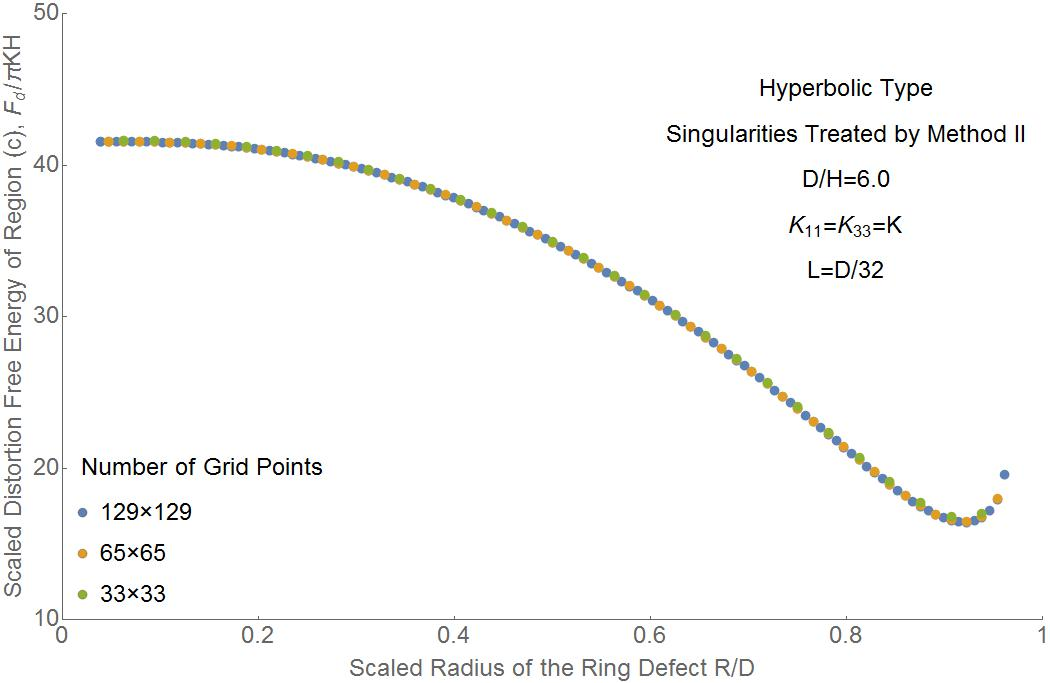
\includegraphics[scale=0.35]{hyperbolicprecise.jpg}\centering
     %\label{fig:hyperbolicprecise}
%\end{subfigure} %

%\begin{subfigure}{.5\textwidth}
%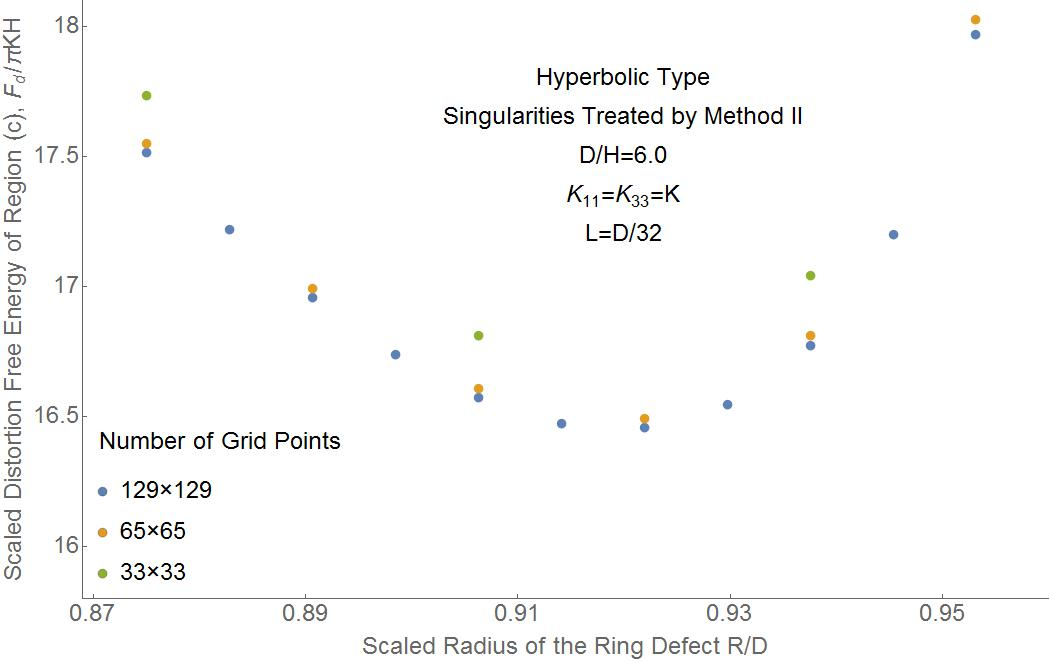
\includegraphics[scale=0.35]{hyperbolicprecise2.jpg}\centering
  %\label{fig:hyperbolicprecise2}
%\end{subfigure}
%\caption{Free energy with singularities treated by method II}
%\label{fig:method2}
%\end{figure}

       Region ($c$) has a characteristic length-scale $H$ ($\sim 10^{-6}m$), and its free energy is denoted by $F_c$.  As the boundary of region (c) has a complex shape, the successive over-relaxation method is used instead of the multi-grid method. We use it to solve Eq.~(\ref{eq:K3}) subject to outer boundary conditions (\ref{eq:theta222})$\sim$(\ref{eq:theta33333}) plus inner boundary conditions given by Eq.~(\ref{eq:theta7}). %\ref{sssec:singularity}.
       %By setting the first derivative of the total free energy to be $0$, we can find the radius corresponding to the stationary point, and the minimal free energy.
       %Note that $F_c$ corresponds to the free energy calculated by method I.
        Figure $7$ shows that the free energy calculated by method II converges more rapidly than that calculated by method I. %, and the energy minimum $F_{c,min}\sim 10^{-16}J$.

      
       It is claimed by B. J. Liang and S. H. Chen that $F_c$ contributes to the universal phase transitions among the four types of structures, while $F_a$ and $F_b$ causes different locations of the transition points for different substances \cite{liang}. However, the validity of this claim is not obvious since the value of  $F_c$ is not exceptionally large compared with the other two. The following is a simple argument that heuristically justify the claim at least for the hyperbolic point-to-hyperbolic ring transition.

      Based on the observation that both $F_a$ and $F_b$ depend linearly on the ring radius,  we simply write the sum of these two as $kR$ ($\sim r\cdot 10^{-16}J$), where $k$ is a constant. Then the equilibrium condition is expressed as

       \begin{equation}\label{eq:F13}
       \frac{\mathrm{d}F_c(R)}{\mathrm{d}R}+k=0.
       \end{equation}
      Assume $R_1$ is the stationary point of $F_c+kR$, in other words, it satisfies Eq. (\ref{eq:F13}). On the other hand, assume that $R_0$ satisfies $F_c^{'}(R_0)=0$. First, we aims at determining the ranges of $D/H$ and $K_{11}/K_{33}$ within which the two stationary points are approximately the same.  For convenience, we consider the difference of the lengths: $\epsilon = R_1-R_0$, such that $|\epsilon/R_0|\ll 1$. Then Eq.~(\ref{eq:F13}) is approximated as

       \begin{equation}\label{eq:F14}
              \epsilon F_c^{''}(R_0)+k=0,
              \end{equation}
      % so
        %\begin{equation}\label{eq:F15}
                    % \epsilon=-\frac{k}{F_c^{''}(R_0)}
                     %\end{equation}
         so
            \begin{equation}\label{eq:k}
             \left|\frac{k}{R_0F_c^{''}(R_0)}\right|\ll 1.
            \end{equation}
Introduce rescaled quantities $r_0=R_0/D$ and $\bar{F}_c=F_c/\pi K_{33}H$, then we have

\begin{equation}\label{eq:bar2}
 \left|\frac{k}{\pi K \bar{F}_c^{''} (r_0)}\cdot\frac{D}{H}\right|\ll 1.
 \end{equation}
 
If Eq.~(\ref{eq:bar2}) is satisfied, then the director fields associated with the local minima for $F_c$ and $(F_a+F_b+F_c)$ are approximately the same. However, the director fields corresponding to the global minima for $F_c$ and $(F_a+F_b+F_c)$ may be different. The following is a detailed explanation.

Denote by $F_P$ and $F_p$ the complete (i.e., $F_a+F_b+F_c$) and partial (i.e., $F_c$) free energies for the hyperbolic point, and denote by $F_R$ and $F_r$ the complete and partial free energies for the hyperbolic ring.  For fixed $K_{11}/K_{33}$, we let the hyperbolic point-to-hyperbolic ring transition point as determined by $F_c$ be $D_0/H_0$; then we have $F_p<F_r$ for $(D/H)<(D_0/H_0)$, $F_p=F_r$ for $(D/H)=(D_0/H_0)$, and $F_p>F_r$ for $(D/H)>(D_0/H_0)$. Similarly, we let the transition point as determined by $(F_a+F_b+F_c)$ be $D_1/H_1$. Because $F_a+F_b=kR$, so the relation $F_R-F_r>F_P-F_p$ is always satisfied and the hyperbolic point-to-hyperbolic ring transition does not switch to a hyperbolic ring-to-hyperbolic point transition, only the {\it location} of the transition point is changed, and we have $(D_1/H_1)>(D_0/H_0)$. 
%, which implies $F_a$ and $F_b$ can change the locations of the transition points.

For the example shown in Fig.~$7$, we performed a second-degree polynomial curve fitting for the data around the stationary point. We have %$r_0=0.913$ and
$\bar{F}_c^{''} (r_0)=1656.93$, which satisfies Eq.~(\ref{eq:bar2}) as it only requires $\bar{F}_c^{''}  (r_0)\gg 20$. That concludes our justification of the claim made by B. J. Liang and S. H. Chen. 


 %which is likely satisfied at least for ring defects since the energy changes sharply near the minimum.




       %\begin{figure}
                         %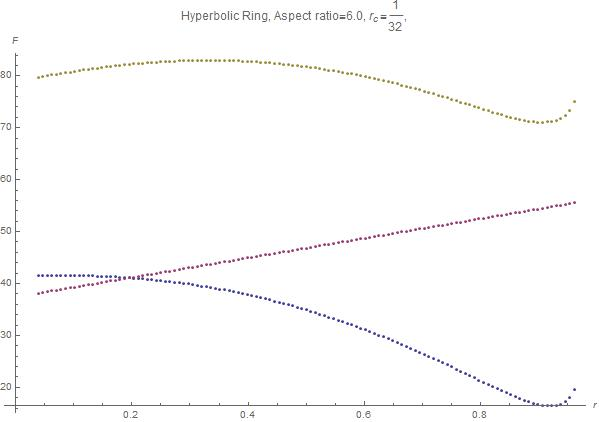
\includegraphics[scale=0.5]{hyperbolictotaltotal.jpg}\centering
                         %caption{Hyperbolic type; aspect radio is 6.0; $K_{11}/K_{33}=1$; $L=1/32$; yellow line: total free energy, violet red line: free energy of region (a) and (b); blue line: free energy of region (c).}
                         %\label{fig:hyperbolictotaltotal}
                       %\end{figure}

%\begin{figure}
                         %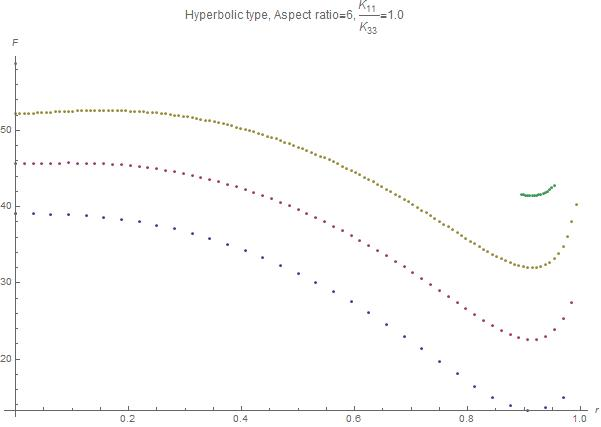
\includegraphics[scale=0.5]{hyperbolicL.jpg}
                         %\caption{Hyperbolic type, aspect radio=6.0, $K_{11}/K_{33}=1$.}
                         %\label{fig:hyperbolicL}
                       %\end{figure}

       % We can see from figure \ref{fig:hyperbolicL} that when $L$ is decreased twice, the free energy is increased by a constant value.
       %\begin{figure}\centering
        %\begin{tikzpicture}
        %\begin{axis}[
            %xmin=0, xmax=6,
            %ymin=0, ymax=3,
            %axis lines=center,
            %axis on top=true,
            %domain=0:1,
            %area style,
           % xlabel=$R/H$,
           % ylabel={$K_{11}/K_{33}$}
           % ]

           % \addplot[color=blue] coordinates {
           % (2.5,0.6)
           % (2.5,3)
           % };
           % \addplot[color=blue] coordinates {
                % (2.5,0.9)
                % (6.0,0.9)
                % };
            % \addplot[color=blue] coordinates {
                %  (1.5,0.6)
                 % (2.5,0.6)
                 % };
            % \addplot[color=blue] coordinates {
                 % (1.5,0.0)
                  %(1.5,0.6)
                 % };
             % \addplot[color=blue] coordinates {
                       % (0.0,0.52)
                      % (1.5,0.52)
                      %  };
           % \node at (100,150) {$I$};
           % \node at (50,30) {$IV$};
           % \node at (400,150) {$II$};
           % \node at (400,30) {$III$};
        % \end{axis}
     % \end{tikzpicture}
     % \caption{I: hyperbolic point, II: hyperbolic ring, III: radial ring, IV: radial point or small ring.}
     % \label{fig:diagram}
     % \end{figure}


The validity of their claim leads to the study of the phase transitions by examining the partial free energy instead of the complete free energy. We calculated the energy minimum $F_{c,min}$ as a function of $D/H$ and $K_{11}/K_{33}$, and obtained the phase diagram as shown in Fig.~\ref{fig:transitiondiagram}. The triple point is approximately at $(D/H, K_{11}/K_{33})=(2.45,0.76)$. Similarly to the phase diagram shown in Ref.~\cite{liang}, Figure~\ref{fig:transitiondiagram} shows a phase transition line between the hyperbolic point and the hyperbolic ring. %Further analysis showed that $I-II$, $I-III$ and $IV-III$ are first order transitions marked by a sudden jump of the radius of the ring defect, which is also consistent with their results.
However, we observe no transition line between the radial point and the radial ring because a radial point gradually expands to a radial ring as $(D/H)$ increases.

       Figure~\ref{fig:transition} shows the hyperbolic point-to-hyperbolic ring transition for $K_{11}=K_{33}=K$. The transition point $(D/H)_c$ is in the range of $2.50660$ to $2.50665$. Near this point,  $\bar{F}_{c,min}~ D/H$ but the proportionality constants are different on the two sides.


     

     \section{Future Work---Defects in the Nematic Bridge}
The closed cylinder is a good geometry to study the effect of the outer boundary on the formation of nematic defects. In experiments, to create such or similar geometry, we put a nematic liquid crystal drop sitting between a solid substrate and a solid top cover slip, surrounded by an environment made of gas or liquid. The resulting geometry made of nematics is called nematic bridge \cite{vogel}. Unfortunately, the nematic bridge is not a perfect cylinder, because the contact angles cannot be $\pi/2$ rad. This requires us to figure out the shape of the outer boundary before studying the defects inside the geometry, under the condition that the shape is not influenced by the defects. The justification of the condition and the method regarding calculations of the shape are as follows.


The total free energy consists of four parts:

\begin{equation}\label{eq:F17}
 F=F_{LC}+F_{g}+F_{surface}+F_{wetting}.
\end{equation}
Here, $F_{LC}$ is the free energy of the nematics, which is given by
\begin{equation}\label{eq:F18}
F_{LC}=F_{b}+F_{d}.
\end{equation}
$F_{g}$ is the gravitational energy of the nematics, which is given by
\begin{equation}\label{eq:F19}
F_{g}=\rho_{LC}gV,
\end{equation}
where $\rho_{LC}$ is the mass density of the nematics. Under the assumption that the bridge is rotational symmetric about the $z$-axis, the free energy of the free surface, $F_{surface}$, is given by
\begin{equation}\label{eq:F20}
 F_{surface}=2\pi\sigma_{LC,en}\int_{-H}^{H}f\sqrt{1+(f^{'})^2}\mathrm{d}z,
\end{equation}
where $f$ is the function of the free surface, $H$ is half of the height, and $\sigma_{LC,en}$ is the appropriate surface tension. $F_{wetting}$ is the wetting energy, and it is given by
 \begin{equation}\label{eq:F21}
  F_{wetting}=-\pi a_1 \Big(f(H)\Big)^2-\pi a_2 \Big(f(-H)\Big)^2,
 \end{equation}
where $a_1$ and $a_2$ are constants; see Refs.~\cite{vogel, vogel2}.  In addition, there is a fixed-volume constraint, i.e.,
\begin{equation}\label{eq:pi}
\pi\int_{-H}^{H}f^2\mathrm{d}\rho=V.
\end{equation}















Small terms can be ignored when we determine the stationary point of this complicated total free energy, therefore it is helpful to compare the magnitude of each term as follows (parameters are given from the measurement of the nematic bridge created in Prof. Fernandez-Nieves' lab \cite{perry}).

(a) Comparison between $F_{g}$ and $F_{surface}$

The relative magnitude between $F_{g}$ and $F_{surface}$ is reflected in the Bond number $Bo$ \cite{sanz}

\begin{equation}\label{eq:Bo}
Bo=\frac{\Delta\rho g D^2}{\sigma_{LC,en}}.
\end{equation}
The magnitudes of the quantities in Eq.~(\ref{eq:Bo}) are approximately
\begin{equation*}%\label{eq:delta}
       \begin{array}{l l l l l}
       \Delta\rho\sim 10^3 \mathrm{kg}\cdot\mathrm{m}^{-3},\\
       g\sim 10\mathrm{m}\cdot\mathrm{s}^{-2},\\
       H\sim 10^{-4}\mathrm{m},\\
       D\sim 10^{-4}\mathrm{m},\\
       \sigma_{LC,en}\sim 10^{-2}\mathrm{kg}\cdot\mathrm{m}\cdot\mathrm{s}^{-2}.
       \end{array}
       \end{equation*}
Therefore $Bo\sim 10^{-2}$, and it implies that %$F_{surface}$ is approximately two orders of magnitude larger than $F_{g}$, therefore 
the shape of the free surface is almost unaffected by the gravity as well as the supportive force from the substrate.

(b) Comparison between $F_{g}$ and $F_{LC}$

We estimated that $F_{LC}\sim
%10^2\cdot 10^{-4}\cdot 10^{-7}\mathrm{J}=
10^{-7}\mathrm{J}$ and $F_{g}\sim
%10^3\cdot 10\cdot 10^{-8}\mathrm{J}=
10^{-4}\mathrm{J}$. Therefore $F_{g}$ is much larger than $F_{LC}$, and the shape of the free surface is unaffected by the nematic defects.
However, note that it is important to remove the divergent free energy at the ``singularities" when we estimate the value of $F_{LC}$, otherwise the calculated distortion free energy can be large enough to change the shape of the free surface.

(c) The magnitude of $F_{wetting}$

The magnitude of $F_{wetting}$ is not important since it only gives us the boundary conditions for the PDE. 

To sum up, even though $f$ exists explicitly or implicitly in all of the four types of free energies, it is mainly affected by $F_{surface}$, $F_{wetting}$ and the fixed-volume constraint. Thus the equilibrium condition with respect to $f$ is derived \cite{vogel}

\begin{equation}\label{eq:f2}
\frac{1}{2}(\frac{f^{''}}{(1+(f^{'})^2)^{3/2}}-\frac{1}{f(1+(f^{'})^2)^{1/2}})=H,
\end{equation}
together with the boundary conditions contributed by $F_{wetting}$


 \begin{equation}\label{eq:f3}
             \left\{
             \begin{array}{l l l}
             \frac{f^{'}(H)}{(1+(f^{'}(H))^2)^{1/2}}=-a_1\\
             \\
             \frac{f^{'}(-H)}{(1+(f^{'}(-H))^2)^{1/2}}=a_2
             \end{array}
             \right.\
        \end{equation}
%The LHS of the Eq.~(\ref{eq:f2}) represents the mean curvature, 
Equation~(\ref{eq:f2}) implies that the free surface has a constant mean curvature, and is named as Delaunay surface \cite{paragoda}. Then the pressure difference $\Delta P$ between the nematics and the environment, i.e., the Laplace pressure, is expressed as \cite{sk}
\begin{equation}\label{eq:delta2}
\Delta P=2\sigma_{LC,en}H.
\end{equation}
%Let $R_1$ and $R_2$ be two principle curvature radii, then the mean curvature is expressed as
%\begin{equation*}
%\frac{1}{2}(\frac{1}{R_{1}}+\frac{1}{R_{2}})
%\end{equation*}
%and $P$ is interpreted as the Laplace pressure, which is the pressure difference between the liquid crystal and the environment. Thus, we have the Laplace equation:
%\begin{equation*}
%P=\sigma_{LC,en}(\frac{1}{R_{1}}+\frac{1}{R_{2}})
%\end{equation*}
In addition, $a_1$ and $a_2$ are related to the contact angles $\theta_1$ and $\theta_2$ by the relations \cite{vogel, vogel2}

 \begin{equation}\label{eq:f5}
             \left\{
             \begin{array}{l l l}
             f^{'}(H)=\cot \theta_1\\
             \\
             f^{'}(-H)=-\cot \theta_2
             \end{array}
             \right.\
        \end{equation}
Therefore, $\theta_1$ and $\theta_2$ are constants as well, which is consistent with the fact that they are determined only by the surface tensions at the interfaces given by the Young equation \cite{lopez}
\begin{equation}\label{eq:sigma}
\sigma_{LC,en}\cos \theta=\sigma_{en,solid}-\sigma_{LC,solid},
\end{equation}
where $\sigma_{LC,en}$, $\sigma_{LC,solid}$, and $\sigma_{en,solid}$ are the surface tensions at the liquid crystal-environment, liquid crystal-solid, and environment-solid interfaces respectively. $f$ satisfies the following equation
%A surface of revolution with constant mean curvature is called the Delaunay surface, and can be further
 \cite{paragoda}

\begin{equation}\label{eq:f7}
f^2\pm \frac{2b_1f}{\sqrt{1+(f^{'})^2}}=\pm b_2^2,
\end{equation}
 where $b_1$ and $b_2$ are positive constants. Solutions to Eq.~(\ref{eq:f7}) describe five different types of Delaunay surfaces: unduloid, sphere, nodoid, cylinder, catenoid. The free surface of a liquid bridge is a part cut from one of them, and can be a cylinder, a ``waist" (a bridge with ``neck") or ``barrel'' (a bridge with ``haunch"); see Refs.~\cite{lopez, lubarda, kra}.

 To determine the equilibrium states of nematic defects, we %minimize the total free energy functional with respect to $\mathbf{n}$ or the corresponding parameter $\theta$, then we can obtain the same
solve Eq.~(\ref{eq:K3}) with homeotropic boundary conditions on the curved free surface. %Because neither $\rho_{LC}$ nor $V$ depends on $\mathbf{n}$, so $F_{g}$ plays no role in this equilibrium condition.

 Experiments in Prof. Fernandez-Nieves' lab show that there is a ring defect when the bridge is ``flat" and a point defect when the bridge is ``tall". Moreover, the defects are of hyperbolic type in the ``waist" and radial type in the ``barrel" \cite{perry}. We are aiming at modifying our algorithm to find the similar results, in particular, modifying the boundary conditions.

 %\subsection {Theorectial Understanding of Nematic Defects in Confined Geometries}
 
 %As discussed in Sec.~\ref{sec:two}, this problem is not a well-defined boundary value problem due to the emergence of unprescribed inner boundary conditions (equivalent to a particular coordinate system). However, its unconstrained counterpart is a well-defined boundary value problem with the free energy density written as
 
 %\begin{equation}\label{eq:m}
 %\mathcal{F}=\frac{K_{11}}{2}(\nabla \cdot \mathbf{m} )^2+\frac{K_{22}}{2}(\mathbf{m}\cdot(\nabla\times\mathbf{m}) )^2+ \frac{K_{33}}{2}\left|\mathbf{m}\times(\nabla\times\mathbf{m}) \right|^2,
 %\end{equation}
 %where the length of $\mathbf{m}$ is unconstrained. One interesting question is whether there exists a correspondence between the ground states of this linear system and the equilibrium states of the original nonlinear system. If the answer is yes, then many of the difficulties can be overcome. So far, this idea may work for the simplest example, i.e., the two-dimensional system with the one-constant approximation for the Frank constants. The details are as follows.
 
 %The director field $\mathbf{m}$ is parametrized as
  %\begin{equation}\label{eq:m2}
  %\mathbf{m}=A(x,y)\cos\theta(x,y)\mathbf{\hat{x}}+A(x,y)\sin\theta(x,y)\mathbf{\hat{y}},
  %\end{equation}
 % where $A(x,y)$ and  $\theta (x,y)$ are the amplitude and phase respectively. The ground state is determined by
  
  %\begin{equation}\label{eq:m3}
             %  \left\{
              %  \begin{array}{l l l}
    
             %   \nabla \cdot \mathbf{m}=0\\
              %  \\
             %   \nabla\times\mathbf{m}=0\\
             %   \end{array}
              %  \right.\
             %   \end{equation}
 % Substitute Eq.~(\ref{eq:m2}) into Eq.~(\ref{eq:m3}), we have the following two first-order PDEs
 
 % \begin{equation}\label{eq:m4}
               %  \left\{
               %  \begin{array}{l l l}
     
             %   \frac{\partial A}{\partial x}+A\frac{\partial \theta}{\partial y}=0\\
              %  \\
              %   A\frac{\partial \theta}{\partial x}-\frac{\partial A}{\partial y}=0\\
              %   \end{array}
              %   \right.\
             %    \end{equation}
 % In the region where $A\neq 0$, Eqs.~(\ref{eq:m4}) satisfy Eq.~(\ref{eq:nnnn22}) which is the equilibrium condition of the original nonlinear system. In the region where $A=0$, the phase $\theta$ is undefined which corresponds to the inner boundaries of the nonlinear system. Thus the correspondence is established. However, one important fact is that the boundary condition for $A$ is unprescribed, and it may be treated as one additional variational parameter. 
 
%  The advantage of this method is that all the physics inside the outer boundary can be fully determined by a set of first-order PDEs and outer boundary conditions. Future work may include a justification of the above method regarding higher-dimensional systems and/or the system with nonidentical Frank constants. 
 


\section{Conclusions}
Defects exist widely in liquid crystals, however, a quantitative study is quite involved. To study the defects of liquid crystals in a closed cylinder, the tensorial representation requires numerous computations, while the vectorial representation needs special treatments of the ``singularities". The study of the nematic bridge problem requires, in addition, modifying the boundary conditions on a curved free surface. Our work will combine computer calculations and mathematical analysis .




\begin{thebibliography}{99}


\bibitem{Mottram}
Mottram, N. J., Newton, C. J.
\newblock {\em Introduction to Q-tensor theory}.
\newblock arXiv preprint arXiv:1409.3542 (2014).

\bibitem{de gennes}
De Gennes P G, Prost J.
\newblock {\em The physics of liquid crystals}.
\newblock Oxford: Clarendon press, 1993.

\bibitem{lubensky}
Chaikin, P. M., Lubensky, T. C.
\newblock {\em Principles of condensed matter physics}.
\newblock Cambridge: Cambridge university press, 2000.

\bibitem{and}
Andrienko, D.
\newblock {\em Introduction to liquid crystals}.
\newblock IMPRS school, Bad Marienberg (2006).

\bibitem{nita}
Popa-Nita, V., Barna, V., Repnik, R., Kralj, S.
\newblock {\em Mixtures Composed of Liquid Crystals and Nanoparticles}.
\newblock 2013.


\bibitem{ball}
Ball, J. M., Zarnescu, A.
\newblock {\em  Orientable and non-orientable line field models for uniaxial nematic liquid crystals}.
\newblock Molecular crystals and liquid crystals, 495(1) (2008), 221-573.



\bibitem{zar}
Zarnescu, A.
\newblock {\em  Topics in the Q-tensor theory of liquid crystals}.
\newblock Topics in mathematical modeling and analysis 7 (2012): 187-252.

\bibitem{berreman}
Berreman, D. W., Meiboom, S.
\newblock {\em Tensor representation of Oseen-Frank strain energy in uniaxial cholesterics}.
\newblock Physical Review A 30.4 (1984): 1955.

\bibitem{mori2}
Mori, H., Gartland Jr, E. C., Kelly, J. R., Bos, P. J.
\newblock {\em Multidimensional director modeling using the Q tensor representation in a liquid crystal cell and its application to the $\pi$ cell with patterned electrodes}.
\newblock Japanese journal of applied physics 38.1R (1999): 135.



\bibitem{zumer}
Kralj, S., $\mathrm{\check{Z}}$umer, S.
\newblock {\em Saddle-splay elasticity of nematic structures confined to a cylindrical capillary}.
\newblock Physical Review E 51.1 (1995): 366.

%\bibitem{oseen}
%Oseen, C. W.
%\newblock {\em  The theory of liquid crystals}.
%\newblock Transactions of the Faraday Society 29.140 (1933): 883-899.

%\bibitem{frank}
%Frank, F. C.
%\newblock {\em  I. Liquid crystals. On the theory of liquid crystals}.
%\newblock Discussions of the Faraday Society 25 (1958): 19-28.


\bibitem{per}
Pergamenshchik, V. M.
\newblock {\em Phenomenological approach to the problem of the K 13 surfacelike elastic term in the free energy of a nematic liquid crystal}.
\newblock Physical Review E 48.2 (1993): 1254.

\bibitem{fati}
Faetti, S.
\newblock {\em Theory of surfacelike elastic contributions in nematic liquid crystals}.
\newblock  Physical Review E 49.5 (1994): 4192.
%\bibitem{trebin}
%Longa, L., Trebin, H. R.
%\newblock {\em  Structure of the elastic free energy for chiral nematic liquid crystals}.
%\newblock Physical Review A 39.4 (1989): 2160.

\bibitem{kleman}
Kleman, M., Lavrentovich, O. D.
\newblock {\em  Topological point defects in nematic liquid crystals}.
\newblock Philosophical Magazine 86.25-26 (2006): 4117-4137.



\bibitem{lavrentovich2}
Lavrentovich, O. D., Pergamenshchik, V. M.
\newblock {\em Disclination loop in Mori-Nakanishi Ansatz: Role of the divergence elasticity}
\newblock Molecular Crystals and Liquid Crystals 299.1 (1997): 301-306.


\bibitem{mori}
Mori, H., Nakanishi, H.
\newblock {\em  On the stability of topologically non-trivial point defects}.
\newblock Journal of the Physical Society of Japan 57.4 (1988): 1281-1286.

\bibitem{lavrentovich}
Lavrentovich, O. D., Ishikawa, T., Terentjev, E. M.
\newblock {\em Disclination loop in Mori-Nakanishi Ansatz: Role of the divergence elasticity}
\newblock Molecular Crystals and Liquid Crystals 299.1 (1997): 301-306.


\bibitem{trebin2}
Penzenstadler, E., Trebin, H. R.
\newblock {\em  Fine structure of point defects and soliton decay in nematic liquid crystals}.
\newblock Journal de Physique 50.9 (1989): 1027-1040.

\bibitem{fukuda}
Fukuda, J. I., Yokoyama, H.
\newblock {\em Stability of a hyperbolic disclination ring in a nematic liquid crystal}.
\newblock Physical Review E 66.1 (2002): 012703.

\bibitem{terentjev}
Terentjev, E. M.
\newblock {\em   Disclination loops, standing alone and around solid particles, in nematic liquid crystals}.
\newblock Physical Review E 51.2 (1995): 1330.

\bibitem{liang}
Liang, B. J., Chen, S. H.
\newblock {\em Director‐configuration diagram for a closed‐cylinder nematic liquid crystal}.
\newblock Journal of applied physics 71.5 (1992): 2189-2194.

\bibitem{pershin}
Pershin, V. K., Klebanov, I. I., Zalmanov, P. B.
\newblock {\em  Point defects and ring defects in a nematic liquid crystal in a cylindrical capillary}.
\newblock Technical Physics 44.7 (1999): 763-766.



\bibitem{press}
Press, W. H., Teukolsky, S. A., Vetterling, W. T., Flannery, B. P.
\newblock {\em Numerical recipes in C (Vol. 2) }.
\newblock Cambridge: Cambridge university press, 1996.

\bibitem{zumer2}
Kralj, S., Virga, E. G., $\mathrm{\check{Z}}$umer, S.
\newblock {\em   Biaxial torus around nematic point defects}.
\newblock Physical Review E 60.2 (1999): 1858.


\bibitem{luca}
De Luca, G., Rey, A. D.
\newblock {\em  Ringlike cores of cylindrically confined nematic point defects}.
\newblock The Journal of chemical physics 126.9 (2007): 094907.

\bibitem{paul2}
Zapotocky M., Goldbart P. M.
\newblock {\em  Topological defects and the short-distance behavior of the structure factor in nematic liquid crystals}.
\newblock arXiv preprint cond-mat/9812235 (1998).

\bibitem{zangwill}
Zangwill, A.
\newblock {\em Modern electrodynamics}.
\newblock  Cambridge University Press, 2013.

\bibitem{paul}
Stone, M., Goldbart, P.
\newblock {\em Mathematics for physics: a guided tour for graduate students}.
\newblock  Cambridge University Press, 2009.

\bibitem{vogel}
Vogel, T. I.
\newblock {\em Stability of a liquid drop trapped between two parallel planes}.
\newblock  SIAM Journal on Applied Mathematics, 1987, 47(3), 516-525.

\bibitem{vogel2}
Vogel, T. I.
\newblock {\em Stability of a liquid drop trapped between two parallel planes II: General contact angles}.
\newblock SIAM Journal on Applied Mathematics, 1989, 49(4), 1009-1028.

\bibitem{sanz}
Sanz, A., Martinez, I.
\newblock {\em Minimum volume for a liquid bridge between equal disks}.
\newblock Journal of Colloid and Interface Science, 1983, 93(1), 235-240.


\bibitem{paragoda}
Paragoda, T.
\newblock {\em Constant Mean Curvature Surfaces of Revolution versus Willmore Surfaces of Revolution: A Comparative Study with Physical Applications}.
\newblock  Doctoral dissertation, Texas Tech University, 2014.

\bibitem{sk}
Skj\ae veland, S. M.
\newblock {\em Derivation of the Laplace equation}.
\newblock  H\o gskolesenteret i Rogaland, 1993.

\bibitem{lopez}
L$\mathrm{\acute{o}}$pez, R.
\newblock {\em  Wetting phenomena and constant mean curvature surfaces with boundary}.
\newblock  Reviews in Mathematical Physics, 2005, 17(07), 769-792.

\bibitem{lubarda}
Lubarda, V. A.
\newblock {\em On the stability of a cylindrical liquid bridge}.
\newblock  Acta Mechanica 226.2 (2014): 233-247.

\bibitem{kra}
Kralchevsky, P., Nagayama, K.
\newblock {\em Particles at fluid interfaces and membranes}.
\newblock Elsevier, Amsterdam, 2001.


\bibitem{perry}
We thank Perry Ellis for helpful discussions.

\bibitem{adkins}
Adkins, C. J.
\newblock {\em Equilibrium thermodynamics}.
\newblock Cambridge University Press, 1983.

\bibitem{sha}
Shahzamanian, M. A., Kadivar, E.
\newblock {\em Disclinations dynamics in confined nematic liquid crystals: strong anchoring}.
\newblock Liquid crystals 33.8 (2006): 941-945.


\bibitem{sha2}
Shahzamanian, M. A., Kadivar, E.
\newblock {\em Annihilation dynamics of the disclination loop in bulk nematic liquid crystals}.
\newblock Molecular Crystals and Liquid Crystals 457.1 (2006): 83-91.
\end{thebibliography}



\end {document}
